
\documentclass{report}

\usepackage{tlatex}
\usepackage{listings}
\usepackage{xcolor}
\usepackage{comment}
\usepackage{fancyhdr}
\usepackage{amssymb}
\usepackage{inputenc}
\usepackage{svg}

\usepackage{tikz}
\usetikzlibrary{automata, positioning, arrows}


% !TeX spellcheck = en_GB 

% Configure fancyhdr
\pagestyle{fancy}
\fancyhf{} % Clear default header and footer

% Header settings
\fancyhead[L]{\nouppercase{\leftmark}} % Chapter number and title on the left
% \fancyhead[C]{Center Header}    % Centered header
\fancyhead[R]{\thepage}     % Right-aligned header

% Footer settings
% \fancyfoot[L]{Left Footer}      % Left-aligned footer
% \fancyfoot[C]{Page \thepage}    % Centered footer with page number
% \fancyfoot[R]{Right Footer}     % Right-aligned footer

% java -cp /home/richard/dev/tla2tex/tla2tools.jar  tla2tex.TeX  book.tex 

\lstset { %
    language=C++,
    backgroundcolor=\color{black!5}, % set backgroundcolor
    basicstyle=\footnotesize,% basic font setting
}

\title{Learning TLA+ by Examples}
\author{Richard Tang}
\date{\today}
\begin{document}
\maketitle
\tableofcontents

\part{Introduction}

\chapter{Motivation}

\section{Catching Problems Early} 

Years ago, I worked on a proprietary low-power processor in an embedded
system. The processor ran a microcode featuring a custom instruction set. To
enter a low-power state, a set (possibly hundreds) of instructions were
executed. These instructions progressively put the system in a lower power state.
For example: Turn off IP A, then turn off IP B, then turn off the power island
to the IPs. To save cost and power, the low-power processor had very limited
debuggability support.\\

An experienced reader may start to notice some red flags.\\

If the microcode attempts to access the memory interface when the power
island has been shut off, the processor will hang. Since the debug power island has
been shut off, the physical hardware debug port is also unavailable, leaving the
developer with \textit{no way} of live debugging problems. At this point,
the developer needs to search through numerous instructions to
catch system constraint violations (invariants) \textit{manually}.\\

As one can imagine, maintaining the microcode was very expensive.
Fortunately, the proprietary low-power processor only had a handful of
instructions, so I created a simulator for this proprietary processor to verify
the microcode before deploying it on-target. The simulator models the processor
states as a state graph, with executed instruction, transitions the state machine
to the next state. At every state, all the invariants are verified. Example
invariants include:
\begin{itemize} 
    \item Accessing memory interface after power off leads to a hang 
    \item Accessing certain register in certain chip revision leads to a hang 
    \item Verify IPs are shut off in the allowed order
\end{itemize}
The verification algorithm was implemented using a \textit{depth-first-search},
providing 100\% microcode coverage before deployment on target.\\

In reality, any system can be modeled as an arbitrary set of states with a
collection of invariants that be true at all times. The complexity of such an
arbitrary system generally grows quadratically as the number of states grows
linearly (eg. in an N-state system, adding state N+1 may introduce N
transitions into the new state). There are many engineering problems with a
large number of states, such as lockless or wait-free data structures,
distributed algorithms, OS schedulers, consensus protocols, and more. As the
number of states grows, the problem becomes more challenging for designers to
reason about.\\

So, how do we produce a system that is \textit{correct by design?} 

\section{The Generalized Problem}

Fast forward to now: I stumbled across TLA+, a formalized solution of what I
was looking for.\\

In the age of big data, vertical scaling is no longer practical. The industry
has been exploring and implementing horizontal scaling solutions for past two
decades. Instead of focusing on increasing clock speed, hardwares vendor has
been focusing on adding more instances of hardware in their design. On the
other hand, software vendors has been designing horizontal scaling solution that
takes advantage of large volume of commodity hardware. There is one slight
problem: Horizontal scaling requires concurrent reasoning, and:\\

\textit{Humans are not good at concurrent reasoning}.\\

Our cognitive system is optimized for sequential reasoning. Enumerating
all scenarios in one's mind to ensure an arbitrary design accommodates all
the corner cases is challenging.\\

Consider a distributed system. The system is a cluster of independently
operating entities, which collectively needs to offer the correct system
behavior. At any given time, nodes in the cluster may receive instructions
out-of-order, crash, recover, etc.\\

Consider a single producer multiple consumer lockless queue. The consumers may
reserve an index in the queue in a certain order but may release it in a
different order. What if one reader is slow, and another reader is superfast
and possibly lapses the slow reader?\\

Consider an OS scheduler with locks. Assume all the processes have the same
priority. Can a process starve the other processes by repeatedly acquiring and
releasing the lock? How do we ensure scheduling is fair?\\

The \textit{anti-pattern} is to keep band-aiding the design until the user stops
filing bug reports. This is never ideal. Per Murphy's law, anything that can go
wrong \textit{will go wrong}, and a hard-to-reproduce bug will come in at the
most inconvenient time. How do we make sure the solution is \textit{correct by
design}? To solve this problem, we must rely on tools to do the reasoning
\textit{for us}.

\section{What is TLA+?}

TLA+ is a \textit{system specification language} to describe a system
without implementation details. TLA+ allows a designer to describe a system as a
set of states with transitions from one state to the next. Designers can
describe invariants that must hold in every state and liveness properties a
sequence of states must satisfy. One of TLA+'s keys is once the system is modeled
as a finite set of states, the states can be \textit{exhaustively} explored
(via breath-first-search) to ensure properties are upheld throughout the entire
state space (either per state or a sequence of states).

\section{About This Book}
This book was initially a set of notes I took while learning TLA+. I decided to
formalize these notes into this short book, which I hope the readers will find
helpful in their TLA+ journey.\newline

The book intends to teach the reader how to write TLA+ specification for their
design to provide confidence in its \textit{correctness}. This book is targeted
to software designers, hardware designers, system architects, and in general
anyone interested in designing correct systems.\newline 

To get the most out of the book, the reader should have general computer science
knowledge. The reader doesn't need to be an expert in a particular language to
understand this book; TLA+ is effectively its own language. This book is
example-driven and will go through designs such as lockless queues, simple task
schedulers, consensus algorithms, etc. Readers will likely enjoy a deeper
insight if there is familiarity with these topics.

\section{How to Use This Book}

This book was designed to be used as a reference, providing examples
and references using TLA+.\\

This book is split into multiple parts, covering TLA+ native notation, PlusCal
(C-like syntax that transpiles down to TLA+ native notation), and rapid
prototyping with TLA+. All examples will follow a similar layout, covering the
problem statement, design, spec, and safety properties.\\

All examples in this book will be presented using TLA+ \textit{mathematical
notation}. Converting between Mathematical and ASCII notation is assumed trivial
due to the one-to-one mapping. Readers are encouraged to consult Table 8 in
\cite{ss} as needed.\\

The last part of the book provides language references and some focused topics.
Readers can use it as general reference. 


\chapter{TLA+ Primer}

\section{Design Intent}

The key insight into TLA+ is modelling a system as a state machine. A simple
digital clock can be represented by two variables, hour and minute and the
number of possible states in a digital clock is $24 * 60 = 1440$.  For example,
10:01 is the next state 10:00 can transition to. Extrapolating further, Asssume
an arbitrarily system described by N variables, each variable having K possible
values such arbitrary system can have up to $N^K$ state.\newline

For every specification, designer can specify \textit{safety} proerty (or
invariants) that must be true in \textit{every} states. For example, in any
state of the digital clock hour \textit{must} be between 0 to 23, or formally
described as $hour \in 0..23$. Similarly, minute must have value between 0 to
59, or $minute \in 0..59$. Examples invariants of a system include: Only one
thread has exclusive access to a critical region, all variables in the system
are within allowable value, resource allocation manager never allocates more
than available resources.\newline

Designer can also specify \textit{liveness} property. These are properties to be
satisfied by a \textit{sequence of state}. One liveness property for the digital
clock could be when the clock is $10:00$, it will eventually become $11:00$
(\textit{$10:00$ leads to $11:00$}). Example liveness property include: a
distributed system eventually converges, the scheduler eventually schedules
every tasks in the task queue, the resource allocation manager fairly allocates
resources. \newline

A TLA+ Spec can be checked by TLC, the model checker. TLC uses
\textit{breath-first search} algorithm to explore \textit{all} states in the
state machine and ensure safety and liveness properties are upheld.\newline

A TLA+ Spec describes the system using \textit{temporal logic}. The syntax may 
appear unfamiliar if one hasn't seen it before, but like any other programming 
language an initiated reader should become familiarized quickly. In this book I
will use 

\section{Requirement}

In this example, we will specify a \textit{digital clock}. The digital clock has
a few simple requirements:
\begin{itemize}
    \item Two variables to represent state: hour and minute
    \item The clock increment one minute at a time
    \item The clock wraps around at midnight (ie. 23:59 transitions to 00:00)
\end{itemize}

\section{Spec}

The \textit{Init} state of such system can be described as: \newline
\begin{tla}
    Init ==
        /\ hour = 0
        /\ minute = 0
\end{tla}
\begin{tlatex}
\@x{\@s{16.4} Init \.{\defeq}}%
\@x{\@s{32.8} \.{\land} hour \.{=} 0}%
\@x{\@s{32.8} \.{\land} minute \.{=} 0}%
\end{tlatex}
 \newline

$\defeq$ is the \textit{defines equal} symbol and $\land$ is the \textit{logical
and} symbol. The above TLA+ syntax can be read as \textit{Init} state is defined
as both hour and minute are both 0.\newline

The spec also always include a $Next$ definition, an \textit{action formula}
describing how the system transition from one state to another. Action formula
contains \textit{primed} variables what happens to the variable in its next
state. The $Next$ action for the digital clock can be defined as:\newline

\begin{tla}
    NextHour ==
        /\ minute = 59 
        /\ hour' = (hour + 1) % 24
        /\ minute' = 0
    NextMinute == 
        /\ minute # 59
        /\ hour' = hour 
        /\ minute' = minute + 1 
    Next ==
        \/ NextMinute
        \/ NextHour
\end{tla}
\begin{tlatex}
\@x{\@s{16.4} NextHour \.{\defeq}}%
\@x{\@s{32.8} \.{\land} minute \.{=} 59}%
\@x{\@s{32.8} \.{\land} hour \.{'} \.{=} ( hour \.{+} 1 ) \.{\%} 24}%
\@x{\@s{32.8} \.{\land} minute \.{'} \.{=} 0}%
\@x{\@s{16.4} NextMinute \.{\defeq}}%
\@x{\@s{32.8} \.{\land} minute \.{\neq} 59}%
\@x{\@s{32.8} \.{\land} hour \.{'} \.{=} hour}%
\@x{\@s{32.8} \.{\land} minute \.{'} \.{=} minute \.{+} 1}%
\@x{\@s{16.4} Next \.{\defeq}}%
\@x{\@s{32.8} \.{\lor} NextMinute}%
\@x{\@s{32.8} \.{\lor} NextHour}%
\end{tlatex}
 \newline

Here's a breakdown of what the spec does:
\begin{itemize}
    \item $Next$ can take $NextMinute$ or $NextHour$
    \item $Next$ takes $NextMinute$ when $minute$ is not 59, next hour is hour, next minute is minute + 1. 
    \item $Next$ takes $NextHour$ when $minute$ is 59, next hour is (hour + 1) modulus 24, next minute set to 0
\end{itemize}

Technically it's possible for $Next$ to take both $NextMinute$ and $NextHour$.
This is not possible in this definition as $NextHour$ and $NextMinute$ are
defined in a \textit{mutually exlusively} fashion.\newline

Finally, the spec itself is formally defined as:\newline
\begin{tla}
    vars == <<hour, minute>>
    Spec ==
        /\ Init
        /\ [][Next]_vars
\end{tla}
\begin{tlatex}
\@x{\@s{16.4} vars\@s{0.63} \.{\defeq} {\langle} hour ,\, minute {\rangle}}%
\@x{\@s{16.4} Spec \.{\defeq}}%
\@x{\@s{32.8} \.{\land} Init}%
\@x{\@s{32.8} \.{\land} {\Box} [ Next ]_{ vars}}%
\end{tlatex}
\newline

$\Box[Next]_{vars}$ deserves some special attention:
\begin{itemize}
    \item $vars$ is defined to be \textit{all} variables in the spec. Different
    combination of these variables constitute the states of the system (eg.
    23:59 and 00:00 are both states in the system).
    \item $\Box[Next]_{vars}$ is a \textit{box-action formula}, where
    \textit{Next} is an action and \textit{vars} is a state function.
    \item $\Box$ operator asserts the formula is always true for every step in the behaviour.
    \item And steps in the behaviour is defined as $[Next]_{vars}$, where $Next$
    describe the action and $vars$ capturing all variables representing the state.
\end{itemize}

%  $,  The formula is true iff every
% successive pair of steps in behaviour is a $[Next]_{vars}$. Finally $Spec$ is
% conjunction between $Init$ and $\Box[Next]_{vars}$. Note \textbf{all} TLA+
% specification follows very similar template. There are situation we will need to
% provide \textit{fairness} description - this will be covered later. \newline

\section{Safety}

Safety property describes invariant that must hold true in every state of
system. A common invariant is \textit{type safety} checks. In a digital clock, 
hour can only be in value between 0 to 23, and minute can only be value of 0 to 59:\newline

\begin{tla}
    Type_OK == 
        /\ hour \in 0..23
        /\ minute \in 0..59
\end{tla}
\begin{tlatex}
\@x{\@s{16.4} Type\_OK \.{\defeq}}%
\@x{\@s{32.8} \.{\land} hour \.{\in} 0 \.{\dotdot} 23}%
\@x{\@s{32.8} \.{\land} minute \.{\in} 0 \.{\dotdot} 59}%
\end{tlatex}

\section{Liveness}

Liveness property verifies certain behavioural across a sequence of state. One
liveness property can be confirming the clock wraps around correctly at
midnight (which involves mutliple states): \newline

\begin{tla}
    Liveness ==
        /\ hour = 23 /\ minute = 59 ~> hour = 0 /\ minute = 0
\end{tla}
\begin{tlatex}
\@x{\@s{16.4} Liveness \.{\defeq}}%
 \@x{\@s{32.8} \.{\land} hour \.{=} 23 \.{\land} minute \.{=} 59 \.{\leadsto}
 hour \.{=} 0 \.{\land} minute \.{=} 0}%
\end{tlatex}
\newline

$\leadsto$ is the \textit{leads to} operator, suggesting something is eventually
true. TLA+ provides a set of formulas that can be used to describe liveness
property.\newline 

To verify liveness, we need to modify the spec slightly to enable
\textit{fairness} to prevent \textit{stuttering}. In plain terms, fairness
ensure \textit{something} always happen in every step, allowing the states to
transition. Without fairness the spec is allowed to \textit{do nothing} as next
step, this means liveness condition may fail because the spec permits the system
to do nothing in perpetuity as next state. Fairness will be covered in more
detailed in later chapter.\newline

\begin{tla}
    Spec ==
        /\ Init
        /\ [][Next]_vars
        /\ WF_vars(Next)
\end{tla}
\begin{tlatex}
\@x{\@s{16.4} Spec \.{\defeq}}%
\@x{\@s{32.8} \.{\land} Init}%
\@x{\@s{32.8} \.{\land} {\Box} [ Next ]_{ vars}}%
\@x{\@s{32.8} \.{\land} {\WF}_{ vars} ( Next )}%
\end{tlatex}
\newline

$WF_{vars}(Next)$ is the fairness qualifier.

% TODO: insert reference here to specifying systems 8.1 

\section{Model Checker}

The TLA+ spec can be verified using TLC model checker. The TLC model checker
runs the spec and verifies all configured safety and liveness properties are
satisfied during execution. To run TLC, we need two things:
\begin{itemize}
    \item clock.tla - the spec itself
    \item clock.cfg - the corresponding configuration file
\end{itemize}

For reference, clock.tla spec is listed below:

\begin{tla}
--------------------------- MODULE clock ----------------------------
EXTENDS Naturals
VARIABLES hour, minute
vars == <<hour, minute>>
Type_OK == 
    /\ hour \in 0..23
    /\ minute \in 0..59
Liveness ==
    /\ hour = 23 /\ minute = 59 ~> hour = 0 /\ minute = 0
Init ==
    /\ hour = 0
    /\ minute = 0
NextMinute ==
    /\ minute = 59 
    /\ hour' = (hour + 1) % 24
    /\ minute' = 0
NextHour == 
    /\ minute # 59
    /\ hour' = hour 
    /\ minute' = minute + 1 
Next ==
    \/ NextMinute
    \/ NextHour
Spec ==
  /\ Init
  /\ [][Next]_vars
  /\ WF_vars(Next)
=============================================================================
\end{tla}
\begin{tlatex}
\@x{}\moduleLeftDash\@xx{ {\MODULE} clock}\moduleRightDash\@xx{}%
\@x{ {\EXTENDS} Naturals}%
\@x{ {\VARIABLES} hour ,\, minute}%
\@x{ vars \.{\defeq} {\langle} hour ,\, minute {\rangle}}%
\@x{ Type\_OK \.{\defeq}}%
\@x{\@s{16.4} \.{\land} hour \.{\in} 0 \.{\dotdot} 23}%
\@x{\@s{16.4} \.{\land} minute \.{\in} 0 \.{\dotdot} 59}%
\@x{ Liveness \.{\defeq}}%
 \@x{\@s{16.4} \.{\land} hour \.{=} 23 \.{\land} minute \.{=} 59 \.{\leadsto}
 hour \.{=} 0 \.{\land} minute \.{=} 0}%
\@x{ Init \.{\defeq}}%
\@x{\@s{16.4} \.{\land} hour \.{=} 0}%
\@x{\@s{16.4} \.{\land} minute \.{=} 0}%
\@x{ NextMinute \.{\defeq}}%
\@x{\@s{16.4} \.{\land} minute \.{=} 59}%
\@x{\@s{16.4} \.{\land} hour \.{'} \.{=} ( hour \.{+} 1 ) \.{\%} 24}%
\@x{\@s{16.4} \.{\land} minute \.{'} \.{=} 0}%
\@x{ NextHour \.{\defeq}}%
\@x{\@s{16.4} \.{\land} minute \.{\neq} 59}%
\@x{\@s{16.4} \.{\land} hour \.{'} \.{=} hour}%
\@x{\@s{16.4} \.{\land} minute \.{'} \.{=} minute \.{+} 1}%
\@x{ Next \.{\defeq}}%
\@x{\@s{16.4} \.{\lor} NextMinute}%
\@x{\@s{16.4} \.{\lor} NextHour}%
\@x{ Spec \.{\defeq}}%
\@x{\@s{8.2} \.{\land}\@s{0.16} Init}%
\@x{\@s{8.2} \.{\land}\@s{0.16} {\Box} [ Next ]_{ vars}}%
\@x{\@s{8.2} \.{\land}\@s{0.16} {\WF}_{ vars} ( Next )}%
\@x{}\bottombar\@xx{}%
\end{tlatex}

The corresponding clock.cfg is listed below: 
\begin{lstlisting}
    SPECIFICATION Spec
    INVARIANTS Type_OK
    PROPERTIES Liveness
\end{lstlisting}

Now run TLC and one should see something like this: 
\begin{lstlisting}
Model checking completed. No error has been found.
...
The depth of the complete state graph search is 1440.
\end{lstlisting}


\part{Examples}

\chapter{Blinking LED}

Let's start with a trivial specification of a blinking LED. The intent of this example 
is to demonstrate the core functionalities of TLA+ specification language.

TODO: briefly talk about tla+ and model checker here.

\section{Requirement}

The LED is represented by a boolean variable that can be either 0 or 1.\newline

... that's it.

\section{Spec}

The specification language may appear alienating as it is mathematically
motivated based on propositional logic. Despite the (possibly) daunting syntax,
designer only need to be familiar with a handful of key operators to start
realizing value using TLA+. This chapter will attempt to describe the example in
exhaustive detail to reduce the learning curve.

The following describe the core portion of the blinking LED spec. 

\begin{tla}
--------------------------- MODULE blinking ----------------------------
VARIABLES b 
vars == <<b>>
Init ==
    /\ b = 0
On == 
    /\ b = 0
    /\ b' = 1
Off == 
    /\ b = 1
    /\ b' = 0
Next ==
    \/ Off 
    \/ On
Spec ==
    /\ Init
    /\ [][Next]_vars
========
\end{tla}
\begin{tlatex}
\@x{}\moduleLeftDash\@xx{ {\MODULE} blinking}\moduleRightDash\@xx{}%
\@x{ {\VARIABLES} b}%
\@x{ vars \.{\defeq} {\langle} b {\rangle}}%
\@x{ Init\@s{2.02} \.{\defeq}}%
\@x{\@s{16.4} \.{\land} b \.{=} 0}%
\@x{ On \.{\defeq}}%
\@x{\@s{18.15} \.{\land} b \.{=} 0}%
\@x{\@s{18.15} \.{\land} b \.{'} \.{=} 1}%
\@x{ Off \.{\defeq}}%
\@x{\@s{15.91} \.{\land} b \.{=} 1}%
\@x{\@s{15.91} \.{\land} b \.{'} \.{=} 0}%
\@x{ Next \.{\defeq}}%
\@x{\@s{16.4} \.{\lor} Off}%
\@x{\@s{16.4} \.{\lor} On}%
\@x{ Spec \.{\defeq}}%
\@x{\@s{16.4} \.{\land} Init}%
\@x{\@s{16.4} \.{\land} {\Box} [ Next ]_{ vars}}%
\@x{}\bottombar\@xx{}%
\end{tlatex}

\begin{itemize}
    \item $\defeq$ is the \textit{defines equal} operator 
    \item $\land$ and $\lor$ are the AND and OR operator. The effect
    of these operator follow the natural definition in English: 
    \begin{itemize}
        \item $C \defeq A \land B$: C is true iff A and B are true
        \item $C \defeq A \lor B$: C is true iff A or B is true
    \end{itemize}
    \item The $'$ operator represents the next state. $b'$ represent b's next state. 
    \item $VARIABLES$ keyword defines a list of variables for the spec. In this case 
    the spec defines a variable $b$ which can be either 0 or 1
    \item $vars$ is typically defined as a shorthand to refer to \textit{all}
    variables in the spec. 
\end{itemize}

With the above definition, we can revisit the Action definitions: $Init$ defines
the initial system state, where b is set to 0.\newline 

$Next$ requires more elaboration. TLA+ specifies the system as a collection of
states with transitions between them. In a simplified sense, the state is
described as a collection of ANDs (eg. system is in state C if both A and B are
true), the ORs then describe the states the system can possibly be in (eg.
system can be in state C OR D). Revisiting the example, the blinking LED has two
states:
\begin{itemize}
    \item $On \defeq b = 0 \land b' = 1$: b switches on 
    \item $Off \defeq = 1 \land b' = 0$: b switches off
\end{itemize}

The system's $Next$ state is defined to be one of these states:\newline
$Next \defeq On \lor Off$.\newline

$\Box[Next]_{vars}$ is a \textbf{Box-Action Formula}, where \textit{Next} is an
action and \textit{vars} is a state function. The formula is true iff every
successive pair of steps in behaviour is a $[Next]_{vars}$. Finally $Spec$ is
conjunction between $Init$ and $\Box[Next]_{vars}$. Note \textbf{all} TLA+
specification follows very similar template. There are situation we will need to
provide \textit{fairness} description - this will be covered later. \newline

In short: this specification describes a two-state state machine where b toggles
between 0 and 1.\newline

Note that b can technically be \textit{anything}. b can be 0, 1, -42, a
dinosaur, etc. TLA+ specifies values of $b$ which are valid in the system.

\section{Safety}

The spec so far only defines the possible states - but the \textit{power} of
TLA+ lies in its \textit{properties} description. Safety properties are
invariants that must hold true in \textit{every} state. An invariant in the
blinking LED example is: 
\begin{tla}
    TypeOK == b \in {0, 1}
\end{tla}
\begin{tlatex}
\@x{\@s{16.4} TypeOK \.{\defeq} b \.{\in} \{ 0 ,\, 1 \}}%
\end{tlatex}

This states the only valid value of b is 0 or 1. If b is ever set to anything
else, the spec is invalid.\newline

Some example safety properties include: Only a single thread have exclusive
access to critical section, number of concurrent reads cannot exceed data
available to be read, etc. 

\section{Liveness}

While safety properties describe invariant that must be upheld in every state,
\textit{Liveness} describe properties of a sequence of states. In the blinking
LED example, a liveness property can be the if b is 0, it eventually becomes 1,
and vice versa. This is described below:
\begin{tla}
    Liveness == 
        /\ b = 0 ~> b = 1
        /\ b = 1 ~> b = 0
\end{tla}
\begin{tlatex}
\@x{\@s{16.4} Liveness \.{\defeq}}%
\@x{\@s{32.8} \.{\land} b \.{=} 0 \.{\leadsto} b \.{=} 1}%
\@x{\@s{32.8} \.{\land} b \.{=} 1 \.{\leadsto} b \.{=} 0}%
\end{tlatex}

It is the author's opinion liveness describes the \textit{design essense} behind
the spec. The key characteristic of a system is described by its
\textit{behaviour} across a series of states. Does a distribute algorithm
eventually converge to a working state? Does a resource manager fairly allocate
resources in all scenarios? Does a scheduler ensure all tasks are eventually
scheduled? These are behaviours that are \textit{cannot} be concluded by looking
at a single state, but across a \textit{sequence of state}. Liveness allows 
designer to express and verify these properties.

\section{Model Checking}

Since the blinking LED is trivially specified, the full specification is
included below. For subsequent chapters only snippet will be included. Please
refer to the accompanied material for full spec source. 

TODO: install toolchain 

TODO: commandline

TODO: using TLC

The following is the content of \textit{blinking.tla}:
\begin{tla}
--------------------------- MODULE blinking ----------------------------
EXTENDS Naturals
VARIABLES b 
vars == <<b>>
TypeOK ==
  /\ b \in {0, 1} 
Liveness == 
    /\ b = 0 ~> b = 1
    /\ b = 1 ~> b = 0
Init ==
  /\ b = 0
Next ==
  \/ /\ b = 0
     /\ b' = 1
  \/ /\ b = 1
     /\ b' = 0
Spec ==
  /\ Init
  /\ [][Next]_vars
  /\ WF_vars(Next)
=============================================================================
\end{tla}
\begin{tlatex}
\@x{}\moduleLeftDash\@xx{ {\MODULE} blinking}\moduleRightDash\@xx{}%
\@x{ {\EXTENDS} Naturals}%
\@x{ {\VARIABLES} b}%
\@x{ vars \.{\defeq} {\langle} b {\rangle}}%
\@x{ TypeOK \.{\defeq}}%
\@x{\@s{8.2} \.{\land} b \.{\in} \{ 0 ,\, 1 \}}%
\@x{ Liveness \.{\defeq}}%
\@x{\@s{16.4} \.{\land} b \.{=} 0 \.{\leadsto} b \.{=} 1}%
\@x{\@s{16.4} \.{\land} b \.{=} 1 \.{\leadsto} b \.{=} 0}%
\@x{ Init \.{\defeq}}%
\@x{\@s{8.2} \.{\land} b \.{=} 0}%
\@x{ Next \.{\defeq}}%
\@x{\@s{8.2} \.{\lor}\@s{1.63} \.{\land} b \.{=} 0}%
\@x{\@s{20.94} \.{\land} b \.{'} \.{=} 1}%
\@x{\@s{8.2} \.{\lor}\@s{1.63} \.{\land} b \.{=} 1}%
\@x{\@s{20.94} \.{\land} b \.{'} \.{=} 0}%
\@x{ Spec \.{\defeq}}%
\@x{\@s{8.2} \.{\land}\@s{0.16} Init}%
\@x{\@s{8.2} \.{\land}\@s{0.16} {\Box} [ Next ]_{ vars}}%
\@x{\@s{8.2} \.{\land}\@s{0.16} {\WF}_{ vars} ( Next )}%
\@x{}\bottombar\@xx{}%
\end{tlatex}

The following is the content of \textit{blinking.cfg}:

\begin{lstlisting}
    SPECIFICATION Spec
    INVARIANTS TypeOK
    PROPERTIES Liveness
\end{lstlisting}

\section{Limitation}

Since TLA+ exhaustively explores all possible state, a linear growth of
variables leads to TLC (temporal logic checker) execution time grows
\textit{exponentially}.This means the specification must be scoped correctly to
limit the state space.\newline

Similarly, if you want to verify concurrent psuedo code implementation in
PlusCal, you can likely at most verify 10s of lines of code.



SPECIFICATION Spec

CONSTANTS
    Servers = {s0, s1, s2}
    \* Servers = {s0, s1}

\* INVARIANTS 
\*     TypeOK
PROPERTIES 
    Liveness


\chapter{Simple Scheduler}

\section{Requirement}

In this section we will define a spec for a simple task scheduler. The task sechdeuler has the following
requirements:
\begin{itemize}
    \item Supporting N execution context (ie. CPUs)
    \item Supporting T number of tasks
    \item Tasks have identical priority and are scheduled coopertively
    \item System has a single global lock
    \item Any task can attempt to acquire the lock, Any task attempting to
    acquire the lock are gauranteed to be scheduled.
    \item If multiple tasks attempt to grab the lock, the tasks will be
    scheduled in lock request order. 
\end{itemize}

\section{Spec}

We will model scheduler using the following variables:\newline
\begin{tla}
Init ==
    /\ cpus = [i \in 0..N-1 |-> ""] 
    /\ ready_q = S2T(Tasks)
    /\ blocked_q = <<>>
    /\ lock_owner = ""
\end{tla}
\begin{tlatex}
\@x{ Init \.{\defeq}}%
 \@x{\@s{16.4} \.{\land} cpus \.{=} [ i \.{\in} 0 \.{\dotdot} N \.{-} 1
 \.{\mapsto}\@w{} ]}%
\@x{\@s{16.4} \.{\land} ready\_q \.{=} S2T ( Tasks )}%
\@x{\@s{16.4} \.{\land} blocked\_q \.{=} {\langle} {\rangle}}%
\@x{\@s{16.4} \.{\land} lock\_owner \.{=}\@w{}}%
\end{tlatex}
\newline

A few things to note:
\begin{itemize}
    \item The system has $N$ executing context, represented as number of CPUs.
    When a task is running, $cpus[k]$ is set to $taskName$. When CPU is idle,
    $cpus[k]$ is set to an empty string. 
    \item $ready\_q$ and $blocked\_q$ are initialized as \textit{ordered tuple},
    due to the cooperative scheduling requirement.
    \item $S2T$ is a macro that converts a set into a ordered tuple. This is to
    accommodate the fact it appears I cannot define tuple in .cfg file.
    \item Finally, the single system lock is represented as $lock\_owner$. 
\end{itemize}

A task can be in three possible state: Ready, Blocked and Running. The $Next$
box-action fomula will define a Ready and Running action, and the implementation
will include related lock contention handling.\newline

\begin{tla}
------- MODULE scheduler ---- 
MoveToReady(k) == 
    /\ cpus[k] # "" 
    /\ lock_owner # cpus[k]
    /\ ready_q' = Append(ready_q, cpus[k]) 
    /\ cpus' = [cpus EXCEPT ![k] = ""]
    /\ UNCHANGED <<lock_owner, blocked_q>>
Lock(k) == 
    \* lock is empty
    \/  /\ cpus[k] # "" 
        /\ lock_owner = ""
        /\ lock_owner' = cpus[k]
        /\ UNCHANGED <<ready_q, cpus, blocked_q>>
    \* someone else has the lock
    \/  /\ cpus[k] # "" 
        /\ lock_owner # ""
        /\ lock_owner # cpus[k] \* cannot double lock
        /\ blocked_q' = Append(blocked_q, cpus[k])
        /\ cpus' = [cpus EXCEPT ![k] = ""]
        /\ UNCHANGED <<ready_q, lock_owner>>
Unlock(k) == 
    /\ cpus[k] # "" 
    /\ lock_owner = cpus[k]
    /\ lock_owner' = ""
    /\ cpus' = [cpus EXCEPT ![k] = ""]
    /\ ready_q' = ready_q \o blocked_q \o <<cpus[k]>>
    /\ blocked_q' = <<>>

Running == 
    \E k \in DOMAIN cpus:
        /\ cpus[k] # "" 
        /\ \/ MoveToReady(k)
           \/ Lock(k)
           \/ Unlock(k)
=============================================================================
\end{tla}
\begin{tlatex}
\@x{}\moduleLeftDash\@xx{ {\MODULE} scheduler}\moduleRightDash\@xx{}%
\@x{ MoveToReady ( k ) \.{\defeq}}%
\@x{\@s{16.4} \.{\land} cpus [ k ] \.{\neq}\@w{}}%
\@x{\@s{16.4} \.{\land} lock\_owner \.{\neq} cpus [ k ]}%
 \@x{\@s{16.4} \.{\land} ready\_q \.{'} \.{=} Append ( ready\_q ,\, cpus [ k ]
 )}%
 \@x{\@s{16.4} \.{\land} cpus \.{'} \.{=} [ cpus {\EXCEPT} {\bang} [ k ]
 \.{=}\@w{} ]}%
 \@x{\@s{16.4} \.{\land} {\UNCHANGED} {\langle} lock\_owner ,\, blocked\_q
 {\rangle}}%
\@x{ Lock ( k ) \.{\defeq}}%
\@x{\@s{20.63}}%
\@y{%
  lock is empty
}%
\@xx{}%
\@x{\@s{20.63} \.{\lor}\@s{4.1} \.{\land} cpus [ k ] \.{\neq}\@w{}}%
\@x{\@s{35.84} \.{\land} lock\_owner \.{=}\@w{}}%
\@x{\@s{35.84} \.{\land} lock\_owner \.{'} \.{=} cpus [ k ]}%
 \@x{\@s{35.84} \.{\land} {\UNCHANGED} {\langle} ready\_q ,\, cpus ,\,
 blocked\_q {\rangle}}%
\@x{\@s{20.63}}%
\@y{%
  someone else has the lock
}%
\@xx{}%
\@x{\@s{20.63} \.{\lor}\@s{4.1} \.{\land} cpus [ k ] \.{\neq}\@w{}}%
\@x{\@s{35.84} \.{\land} lock\_owner \.{\neq}\@w{}}%
\@x{\@s{35.84} \.{\land} lock\_owner \.{\neq} cpus [ k ]}%
\@y{%
  cannot double lock
}%
\@xx{}%
 \@x{\@s{35.84} \.{\land} blocked\_q \.{'}\@s{5.22} \.{=} Append ( blocked\_q
 ,\, cpus [ k ] )}%
 \@x{\@s{35.84} \.{\land} cpus \.{'} \.{=} [ cpus {\EXCEPT} {\bang} [ k ]
 \.{=}\@w{} ]}%
 \@x{\@s{35.84} \.{\land} {\UNCHANGED} {\langle} ready\_q ,\, lock\_owner
 {\rangle}}%
\@x{ Unlock ( k ) \.{\defeq}}%
\@x{\@s{16.4} \.{\land} cpus [ k ] \.{\neq}\@w{}}%
\@x{\@s{16.4} \.{\land} lock\_owner \.{=} cpus [ k ]}%
\@x{\@s{16.4} \.{\land} lock\_owner \.{'} \.{=}\@w{}}%
 \@x{\@s{16.4} \.{\land} cpus \.{'} \.{=} [ cpus {\EXCEPT} {\bang} [ k ]
 \.{=}\@w{} ]}%
 \@x{\@s{16.4} \.{\land} ready\_q \.{'} \.{=} ready\_q \.{\circ} blocked\_q
 \.{\circ} {\langle} cpus [ k ] {\rangle}}%
\@x{\@s{16.4} \.{\land} blocked\_q \.{'} \.{=} {\langle} {\rangle}}%
\@pvspace{8.0pt}%
\@x{ Running \.{\defeq}}%
\@x{\@s{16.4} \E\, k \.{\in} {\DOMAIN} cpus \.{:}}%
\@x{\@s{27.72} \.{\land} cpus [ k ] \.{\neq}\@w{}}%
\@x{\@s{27.72} \.{\land} \.{\lor} MoveToReady ( k )}%
\@x{\@s{38.83} \.{\lor} Lock ( k )}%
\@x{\@s{38.83} \.{\lor} Unlock ( k )}%
\@x{}\bottombar\@xx{}%
\end{tlatex}

\section{Safety}

\section{Liveness}

I believe this is the most important part of cooperative scheduler design. While
the scheduler can't \textit{force} a task to relinquish a lock (the scheduler
doesn't dictate when the task is \textit{done}), the scheduler can ensure
scheduling fairness by scheduling the next lock requester intsead of the task 
that just relinquished the lock.\newline

\begin{tla}
----- MODULE scheduler ---- 
Liveness == 
    \A t \in Tasks:
        LET 
            b == {x \in DOMAIN blocked_q : blocked_q[x] = t}
        IN 
            /\ b # {} ~> b = {}
==========
\end{tla}
\begin{tlatex}
\@x{}\moduleLeftDash\@xx{ {\MODULE} scheduler}\moduleRightDash\@xx{}%
\@x{ Liveness \.{\defeq}}%
\@x{\@s{16.4} \A\, t \.{\in} Tasks \.{:}}%
\@x{\@s{27.72} \.{\LET}}%
 \@x{\@s{44.12} b \.{\defeq} \{ x \.{\in} {\DOMAIN} blocked\_q \.{:}
 blocked\_q [ x ] \.{=} t \}}%
\@x{\@s{27.72} \.{\IN}}%
\@x{\@s{44.12} \.{\land} b \.{\neq} \{ \} \.{\leadsto} b \.{=} \{ \}}%
\@x{}\bottombar\@xx{}%
\end{tlatex}
\newline

The formula defines set b to be either an empty set or a set of one task. Assume
a set of \{"p0", "p1", "p2\}. Possible value of b include: \{\}, \{"p0"\},
\{"p1"\} and \{"p2"\}. The fomula then states an non empty set of b leads to an
\textit{empty set} of b. In other words: \newline

\textit{If a task ever becomes blocked, it will eventually become unblocked}.\newline

However, when we actually run the model checker, we will find the liveness
property is \textit{violated}. The failure scenario is basically one task
holding onto the lock in one CPU, while the scheduler repeatedly
schedule/deschedule a separate task in another CPU. While this is perfectly
allowed, the model checker detects a possible path for the the system to trap in
a local state and fail the liveness property.\newline 

Perhaps not surprisingly, if you construct similar liveness property to verify 
a task is \textit{eventually} always scheduled, it will also fail. The model
checker will provide a counter case where a task is never scheduled because
another task is repeatedly acquire/release the global lock.\newline

We need \textit{Strong Fairness} to solve this problem:
\begin{tla}
----- MODULE scheduler ---- 
L ==
    \A t \in Tasks :
        \A n \in 0..(N-1) :
            WF_vars(HoldingLock(t) /\ Unlock(n))
Spec ==
  /\ Init
  /\ [][Next]_vars
  /\ WF_vars(Next)
  /\ L 
======= 
\end{tla}
\begin{tlatex}
\@x{}\moduleLeftDash\@xx{ {\MODULE} scheduler}\moduleRightDash\@xx{}%
\@x{ L \.{\defeq}}%
\@x{\@s{14.47} \A\, t \.{\in} Tasks \.{:}}%
\@x{\@s{25.79} \A\, n \.{\in} 0 \.{\dotdot} ( N \.{-} 1 ) \.{:}}%
\@x{\@s{37.11} {\WF}_{ vars} ( HoldingLock ( t ) \.{\land} Unlock ( n ) )}%
\@x{ Spec \.{\defeq}}%
\@x{\@s{8.2} \.{\land}\@s{0.16} Init}%
\@x{\@s{8.2} \.{\land}\@s{0.16} {\Box} [ Next ]_{ vars}}%
\@x{\@s{8.2} \.{\land}\@s{0.16} {\WF}_{ vars} ( Next )}%
\@x{\@s{8.2} \.{\land}\@s{0.16} L}%
\@x{}\bottombar\@xx{}%
\end{tlatex}
\newline

Fairness ensures that we are never stuck in a repeated state.



\chapter{Selective Retransmit}

Assume client device that playsback a video stream. Structurelly, a video is
composed of frames, frames are then segmented into packets to stream across a 
network. The client device recombines the packets into a frame, then sequence
the frame to playback the video.\newline

However, network is not-deterministic. Depending on the route the packets take
to get to the client, they may arrive out-of-order. The client may need to
maintain a receive buffer for the packets, re-order the packets back into
sequence before pushing the packets down to decoding engine.\newline

The network may also drop packets if any of the switches gets too busy. In the
case of a packet drop, the client has a few options. The client can either
discard the frame and let the decoding engine downstream to deal with it (which
may ressult in  visible artifacts during play back). The client can request the
whole frame to be re-sent, which results in additional bandwidith consumption.
The client can selectively request the missing packet to be retransmited, which
will minimize additional bandwidth consumption, but increases implementation 
complexity.\newline 

In this chapter, we will implement a simple selective retransmit
algorithm.\newline

\begin{center}

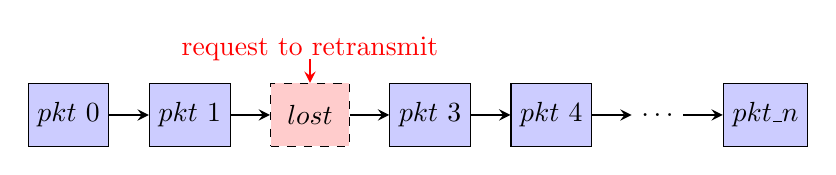
\begin{tikzpicture}[
    packet/.style={rectangle, draw, fill=blue!20, minimum width=1cm, minimum height=0.8cm},
    missing/.style={rectangle, draw, dashed, fill=red!20, minimum width=1cm, minimum height=0.8cm},
    arrow/.style={->, >=stealth, thick}
]

    % Draw packets
    \node[packet] (p0) at (0,0) {\(pkt\ 0\)};
    \node[packet, right=0.5cm of p0] (p2) {\(pkt\ 1\)};
    \node[missing, right=0.5cm of p2] (missing1) {\(lost\)};
    \node[packet, right=0.5cm of missing1] (p4) {\(pkt\ 3\)};
    \node[packet, right=0.5cm of p4] (p5) {\(pkt\ 4\)};
    \node[right=0.5cm of p5] (dots) {\(\dots\)}; % Just dots, no box
    \node[packet, right=0.5cm of dots] (pn) {\(pkt\_n\)};

    % Draw arrows between packets
    \draw[arrow] (p0.east) -- (p2.west);
    \draw[arrow] (p2.east) -- (missing1.west);
    \draw[arrow] (missing1.east) -- (p4.west);
    \draw[arrow] (p4.east) -- (p5.west);
    \draw[arrow] (p5.east) -- (dots);
    \draw[arrow] (dots) -- (pn.west);

    % Add arrow pointing to "lost" with caption
    \draw[arrow, red] ([yshift=0.3cm] missing1.north) -- (missing1.north) 
        node[midway, above, text=red] {request to retransmit};

\end{tikzpicture}

\end{center}

\section{Requirement}

Since packets may arrive out-of-order, the server stamps the packets with
sequence number to allow the client to order the packets as they arrive.
Once the client has a set of ordered packets, it moves the packets from the 
receive buffer into the decoding engine to be displayed.\newline

The video packets are often sent to client via unreliable channel to minimize
network overhead and latency. The client sends acknowledgement back to the
server via to acknowledge the received packet. This indicates to the server it
can send more video data to the client. The acknowlegements are not latency
sensitive in nature, and take up a very small proportion of bandwidth, so they
are transported through reliable channel.\newline

The following illustrates a re-ordering scenario:
\begin{center}
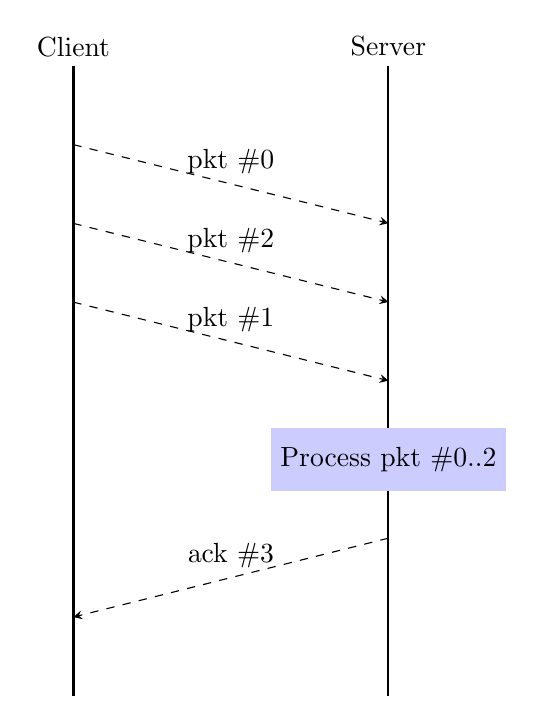
\begin{tikzpicture}[
    lifeline/.style={thick},
    message/.style={->, >=stealth, dashed},
    activation/.style={rectangle, fill=blue!20, minimum width=0.5cm, minimum height=0.8cm} ]

    % Define lifelines
    \node[] (client) at (0,0) {Client};
    \node[] (server) at (4,0) {Server};
    % \node[] (database) at (8,0) {Database};

    % Draw lifelines
    \draw[lifeline] (client.south) -- ++(0,-8);
    \draw[lifeline] (server.south) -- ++(0,-8);
    % \draw[lifeline] (database.south) -- ++(0,-8);

    % Draw messages
    \draw[message] ([yshift=-1cm] client.south) -- node[above] {pkt \#0} ([yshift=-2cm] server.south);
    \draw[message] ([yshift=-2cm] client.south) -- node[above] {pkt \#2} ([yshift=-3cm] server.south);
    \draw[message] ([yshift=-3cm] client.south) -- node[above] {pkt \#1} ([yshift=-4cm] server.south);
    % \draw[message] ([yshift=-2cm] server.south) -- node[above] {query} ([yshift=-2cm] database.south);
    % \draw[message] ([yshift=-3cm] database.south) -- node[above] {response} ([yshift=-3cm] server.south);
    \draw[message] ([yshift=-6cm] server.south) -- node[above] {ack \#3} ([yshift=-7cm] client.south);

    % \draw[message] ([yshift=-5cm] server.south) to[out=-90, in=-90, looseness=1.5] node[above] {ack \#3} ([yshift=-6cm] server.south);
    % \draw[message] ([yshift=-1cm] server.south) to[out=-90, in=-90, looseness=1.5] node[midway, above] {ack \#3} ([yshift=-2cm] server.south);

    % Draw activations
    \node[activation] at ([yshift=-5cm] server.south) {Process pkt \#0..2};
    % \node[activation] at ([yshift=-2.5cm] database.south) {};

    % \draw[arrow, out=120, in=60, looseness=8] (server.west) to node[above] {} (server.east);
    % \begin{umlcallself}[op=c1, return=0]{b} 
    % \draw[message] ([yshift=-1cm] server.south) to[out=-100, in=100, looseness=1.5] node[midway, above] {ack \#3} ([yshift=-2cm] server.south);

    % Optional: Add dashed lines for return messages
    % \draw[dashed] ([yshift=-3cm] database.south) -- ++(0,-1);
    % \draw[dashed] ([yshift=-4cm] server.south) -- ++(0,-1);
 
\end{tikzpicture}
\end{center}


\section{Spec}



% \begin{document}

\chapter{Raft Consensus Protocol}

Raft is a consensus algorithm that enables a cluster of nodes to agree on a
collective state even in the presence of failures. An application of Raft is
a database replication protocol. With a replication factor of 3 (eg. data is
replicated across 3 nodes) and a hard drive failure rate of 0.81\% per year, the
possibility of total failure where the entire replication group goes down is
$1-0.0081^3 = 99.9999\%$ uptime \cite{backblaze}.\\

This chapter implements only the leader election portion of the protocol to
limit the scope of the discussion. For a full description of the Raft
protocol, please refer to the original paper \cite{raft}.\\

\section{Design}

We will briefly describe Raft and its leadership election process below: 
\begin{itemize}
    \item A Raft cluster has N nodes, the cluster works collectively as a
    \textit{system} to offer some service
    \item Each node can be in one of three possible states: Follower, Candidate, Leader
    \item During normal operations, a cluster of N nodes has a single leader
    and N-1 followers
    \item The leader handles all the client interactions. Requests sent to followers will be 
    redirected to the leader
    \item The leader regularly sends a heartbeat to the follower, indicating its
    alive
    \item If a follower fails to receive a heartbeat from the leader after
    timeout, it will become a candidate, vote for itself, and campaign to be
    leader
    \item A candidate who collects the majority of the vote becomes the leader
    \item If multiple candidates are campaigning and a split vote happens,
    candidates will eventually declare an election timeout and start a new round of
    election
    \item The cluster can have multiple leaders due to unfavorable network conditions, 
    but the leaders must be on different terms 
    \item A newly elected leader will send a heartbeat to other nodes to establish 
    leadership 
    \item All requests and responses include the sender's term, allowing the
    receiver to react accordingly
\end{itemize}

The protocol also included a description of log synchronization, state
recovery, and more. Many details are omitted in this chapter to reduce modeling
costs. The N nodes in the cluster operate \textit{independently} following the
above heuristics. Hopefully, this highlights the complexity of verifying the
correctness of the protocol.\newline

The following illustrates the state diagram of one node in the cluster:\newline
\begin{center}
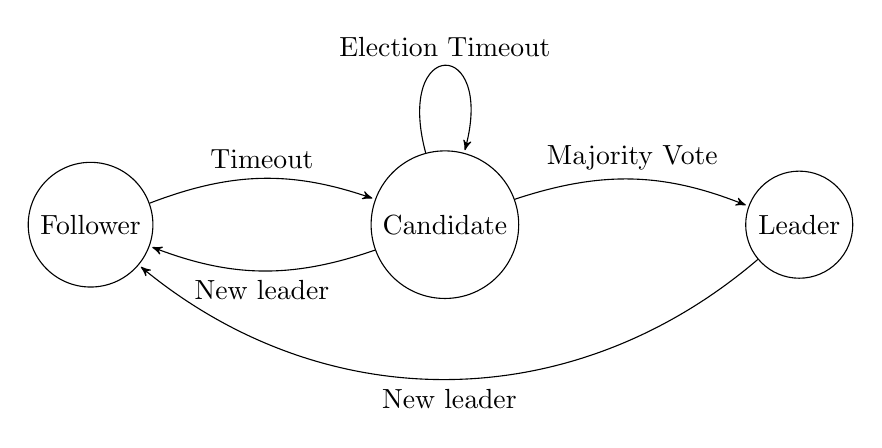
\begin{tikzpicture}[>=stealth',shorten >=1pt,auto,node distance=4.5cm]
  \node[state]  (f)                {Follower};
  \node[state]  (c) [right of=f]  {Candidate};
  \node[state]  (l) [right of=c]  {Leader};

  \path[->]          (f)  edge   [bend left=20]   node {Timeout} (c);
  \path[->]          (c)  edge   [bend left=20]   node {New leader} (f);

  \path[->]          (c)  edge   [bend left=20]   node {Majority Vote} (l);
  \path[->]          (l)  edge   [bend left=40]   node {New leader} (f);
  \path[->] (c) edge [loop above] node {Election Timeout} (c);

\end{tikzpicture}
\end{center}

\section{Spec}

The following implements the skeleton portion of the leader election
protocol:\newline

\begin{tla}
Init ==
    /\ state = [s \in Servers |-> "Follower"]
    /\ messages = {} 
    /\ voted_for = [s \in Servers |-> ""]
    /\ vote_granted = [s \in Servers |-> {}]
    /\ vote_requested = [s \in Servers |-> 0]
    /\ term = [s \in Servers |-> 0]

RequestVoteSet(i) == {
    [fSrc |-> i, fDst |-> s, fType |-> "RequestVoteReq", fTerm |-> term[i]] 
        : s \in Servers \ {i}
}

Campaign(i) == 
    /\ vote_requested[i] = 0
    /\ vote_requested' = [vote_requested EXCEPT ![i] = 1]
    /\ messages' = messages \cup RequestVoteSet(i) 
    /\ UNCHANGED <<state, term, vote_granted, voted_for>>

KeepAliveSet(i) == {
    [fSrc |-> i, fDst |-> s, fType |-> "AppendEntryReq", fTerm |-> term[i]] 
        : s \in Servers \ {i}
}

Leader(i) == 
    /\ state[i] = "Leader"
    /\ messages' = messages \cup KeepAliveSet(i) 
    /\ UNCHANGED <<state, voted_for, term, vote_granted, vote_requested>>

BecomeLeader(i) ==
    /\ Cardinality(vote_granted[i]) > Cardinality(Servers) \div 2
    /\ state' = [state EXCEPT ![i] = "Leader"]
    /\ UNCHANGED <<messages, voted_for, 
        term, vote_granted, vote_requested>>

Candidate(i) == 
    /\ state[i] = "Candidate"
    /\ \/ Campaign(i)
       \/ BecomeLeader(i)
       \/ Timeout(i)

Follower(i) == 
    /\ state[i] = "Follower"
    /\ Timeout(i)

Receive(msg) == 
    \/ /\ msg.fType = "AppendEntryReq"
       /\ AppendEntryReq(msg) 
    \/ /\ msg.fType = "AppendEntryResp"
       /\ AppendEntryResp(msg) 
    \/ /\ msg.fType = "RequestVoteReq"
       /\ RequestVoteReq(msg) 
    \/ /\ msg.fType = "RequestVoteResp"
       /\ RequestVoteResp(msg) 

Next == 
    \/ \E i \in Servers : 
          \/ Leader(i) 
          \/ Candidate(i)
          \/ Follower(i)
    \/ \E msg \in messages : Receive(msg)
\end{tla}
\begin{tlatex}
\@x{ Init \.{\defeq}}%
 \@x{\@s{16.4} \.{\land} state \.{=} [ s \.{\in} Servers
 \.{\mapsto}\@w{Follower} ]}%
\@x{\@s{16.4} \.{\land} messages \.{=} \{ \}}%
 \@x{\@s{16.4} \.{\land} voted\_for \.{=} [ s \.{\in} Servers \.{\mapsto}\@w{}
 ]}%
 \@x{\@s{16.4} \.{\land} vote\_granted \.{=} [ s \.{\in} Servers \.{\mapsto}
 \{ \} ]}%
 \@x{\@s{16.4} \.{\land} vote\_requested \.{=} [ s \.{\in} Servers \.{\mapsto}
 0 ]}%
\@x{\@s{16.4} \.{\land} term \.{=} [ s \.{\in} Servers \.{\mapsto} 0 ]}%
\@pvspace{8.0pt}%
\@x{ RequestVoteSet ( i ) \.{\defeq} \{}%
 \@x{\@s{16.4} [ fSrc \.{\mapsto} i ,\, fDst \.{\mapsto} s ,\, fType
 \.{\mapsto}\@w{RequestVoteReq} ,\, fTerm \.{\mapsto} term [ i ] ]}%
\@x{\@s{28.69} \.{:} s \.{\in} Servers \.{\,\backslash\,} \{ i \}}%
\@x{ \}}%
\@pvspace{8.0pt}%
\@x{ Campaign ( i ) \.{\defeq}}%
\@x{\@s{16.4} \.{\land} vote\_requested [ i ] \.{=} 0}%
 \@x{\@s{16.4} \.{\land} vote\_requested \.{'} \.{=} [ vote\_requested
 {\EXCEPT} {\bang} [ i ] \.{=} 1 ]}%
 \@x{\@s{16.4} \.{\land} messages \.{'} \.{=} messages \.{\cup} RequestVoteSet
 ( i )}%
 \@x{\@s{16.4} \.{\land} {\UNCHANGED} {\langle} state ,\, term ,\,
 vote\_granted ,\, voted\_for {\rangle}}%
\@pvspace{8.0pt}%
\@x{ KeepAliveSet ( i ) \.{\defeq} \{}%
 \@x{\@s{16.4} [ fSrc \.{\mapsto} i ,\, fDst \.{\mapsto} s ,\, fType
 \.{\mapsto}\@w{AppendEntryReq} ,\, fTerm \.{\mapsto} term [ i ] ]}%
\@x{\@s{28.69} \.{:} s \.{\in} Servers \.{\,\backslash\,} \{ i \}}%
\@x{ \}}%
\@pvspace{8.0pt}%
\@x{ Leader ( i ) \.{\defeq}}%
\@x{\@s{16.4} \.{\land} state [ i ] \.{=}\@w{Leader}}%
 \@x{\@s{16.4} \.{\land} messages \.{'} \.{=} messages \.{\cup} KeepAliveSet (
 i )}%
 \@x{\@s{16.4} \.{\land} {\UNCHANGED} {\langle} state ,\, voted\_for ,\, term
 ,\, vote\_granted ,\, vote\_requested {\rangle}}%
\@pvspace{8.0pt}%
\@x{ BecomeLeader ( i ) \.{\defeq}}%
 \@x{\@s{16.4} \.{\land} Cardinality ( vote\_granted [ i ] ) \.{>} Cardinality
 ( Servers ) \.{\div} 2}%
 \@x{\@s{16.4} \.{\land} state \.{'} \.{=} [ state {\EXCEPT} {\bang} [ i ]
 \.{=}\@w{Leader} ]}%
\@x{\@s{16.4} \.{\land} {\UNCHANGED} {\langle} messages ,\, voted\_for ,\,}%
\@x{\@s{20.5} term ,\, vote\_granted ,\, vote\_requested {\rangle}}%
\@pvspace{8.0pt}%
\@x{ Candidate ( i ) \.{\defeq}}%
\@x{\@s{16.4} \.{\land} state [ i ] \.{=}\@w{Candidate}}%
\@x{\@s{16.4} \.{\land} \.{\lor} Campaign ( i )}%
\@x{\@s{16.4} \.{\lor} BecomeLeader ( i )}%
\@x{\@s{16.4} \.{\lor} Timeout ( i )}%
\@pvspace{8.0pt}%
\@x{ Follower ( i ) \.{\defeq}}%
\@x{\@s{16.4} \.{\land} state [ i ] \.{=}\@w{Follower}}%
\@x{\@s{16.4} \.{\land} Timeout ( i )}%
\@pvspace{8.0pt}%
\@x{ Receive ( msg ) \.{\defeq}}%
\@x{\@s{16.4} \.{\lor} \.{\land} msg . fType \.{=}\@w{AppendEntryReq}}%
\@x{\@s{16.4} \.{\land} AppendEntryReq ( msg )}%
\@x{\@s{16.4} \.{\lor} \.{\land} msg . fType \.{=}\@w{AppendEntryResp}}%
\@x{\@s{16.4} \.{\land} AppendEntryResp ( msg )}%
\@x{\@s{16.4} \.{\lor} \.{\land} msg . fType \.{=}\@w{RequestVoteReq}}%
\@x{\@s{16.4} \.{\land} RequestVoteReq ( msg )}%
\@x{\@s{16.4} \.{\lor} \.{\land} msg . fType \.{=}\@w{RequestVoteResp}}%
\@x{\@s{16.4} \.{\land} RequestVoteResp ( msg )}%
\@pvspace{8.0pt}%
\@x{ Next \.{\defeq}}%
\@x{\@s{16.4} \.{\lor} \E\, i \.{\in} Servers \.{:}}%
\@x{\@s{16.4} \.{\lor} Leader ( i )}%
\@x{\@s{16.4} \.{\lor} Candidate ( i )}%
\@x{\@s{16.4} \.{\lor} Follower ( i )}%
\@x{\@s{16.4} \.{\lor} \E\, msg \.{\in} messages \.{:} Receive ( msg )}%
\end{tlatex}

\begin{itemize}
    \item \textit{Next} either picks a server to make progress, or picks a
    message in the message pool to process. Message processing is done by
    \textit{Receive}, handling is state agnostic
    \item \textit{message} is defined to be a set that holds a collection of functions, where 
    each function is a message with source, destination, type, and more specified
    \item \textit{voted\_for} tracks who a given node previously voted for.
    This prevents a node from voting more than once
    \item \textit{vote\_granted} tracks how many votes a candidate has received
    \item \textit{vote\_requested} tracks if a node has already issued a request
    vote to its peers
    \item \textit{Follower} either Receive or Timeout and campaign to be a leader
    \item \textit{Candidate} campaigns to be a leader, and becomes one if it has
    enough vote. Failing to collect enough votes, \textit{Candidate} start a new
    election on a new term. It can also receive a request with a higher term and
    transition to be a \textit{Follower}.
    \item \textit{Leader} will establish its leadership by sending
    \textit{AppepndEntryReq} to all its peers
\end{itemize}

 \textit{Spec} implements four messages AppendEntry request/response, RequestVote
request/response. Handling for all messages is similar in structure. In
this chapter, we will look at \textit{RequestVoteReq} only. Readers are
encouraged to check the remaining definition as an exercise:\newline

\begin{tla}
RequestVoteReq(msg) == 
    LET 
        i == msg.fDst
        j == msg.fSrc
        type == msg.fType
        t == msg.fTerm
    IN 
        \* haven't voted, or whom we voted re-requested
        \/ /\ t = term[i]
           /\ \/ voted_for[i] = j 
              \/ voted_for[i] = ""
           /\ voted_for' = [voted_for EXCEPT ![i] = j]
           /\ messages' = AddMessage([fSrc |-> i, 
                                        fDst |-> j, 
                                        fType |-> "RequestVoteResp",
                                        fTerm |-> t, 
                                        fSuccess |-> 1],
                                        RemoveMessage(msg, messages))
           /\ UNCHANGED <<state, term, vote_granted, 
                vote_requested, establish_leadership >>
        \* already voted for someone else
        \/ /\ t = term[i]
           /\ voted_for[i] # j 
           /\ voted_for[i] # ""
           /\ messages' = AddMessage([fSrc |-> i, 
                                        fDst |-> j, 
                                        fType |-> "RequestVoteResp",
                                        fTerm |-> t, 
                                        fSuccess |-> 0],
                                        RemoveMessage(msg, messages))
            /\ UNCHANGED <<state, voted_for, term, 
                vote_granted, vote_requested, establish_leadership>>
        \/  /\ t < term[i]
            /\ messages' = AddMessage([fSrc |-> i, 
                                        fDst |-> j, 
                                        fType |-> "RequestVoteResp",
                                        fTerm |-> term[i], 
                                        fSuccess |-> 0],
                                        RemoveMessage(msg, messages))
            /\ UNCHANGED <<state, voted_for, term, 
                vote_granted, vote_requested, establish_leadership>>
        \* revert to follower
        \/  /\ t > term[i]
            /\ state' = [state EXCEPT ![i] = "Follower"]
            /\ term' = [term EXCEPT ![i] = t]
            /\ voted_for' = [voted_for EXCEPT ![i] = j]
            /\ vote_granted' = [vote_granted EXCEPT ![i] = {}]
            /\ vote_requested' = [vote_requested EXCEPT ![i] = 0]
            /\ establish_leadership' = [establish_leadership EXCEPT ![i] = 0]
            /\ messages' = AddMessage([fSrc |-> i, 
                                        fDst |-> j, 
                                        fType |-> "RequestVoteResp",
                                        fTerm |-> t, 
                                        fSuccess |-> 1],
                                        RemoveMessage(msg, messages))
\end{tla}
\begin{tlatex}
\@x{ RequestVoteReq ( msg ) \.{\defeq}}%
\@x{\@s{16.4} \.{\LET}}%
\@x{\@s{32.8} i \.{\defeq} msg . fDst}%
\@x{\@s{32.8} j \.{\defeq} msg . fSrc}%
\@x{\@s{32.8} type \.{\defeq} msg . fType}%
\@x{\@s{32.8} t \.{\defeq} msg . fTerm}%
\@x{\@s{16.4} \.{\IN}}%
\@x{\@s{32.8}}%
\@y{%
  haven't voted, or whom we voted re-requested
}%
\@xx{}%
\@x{\@s{32.8} \.{\lor} \.{\land} t \.{=} term [ i ]}%
\@x{\@s{32.8} \.{\land} \.{\lor} voted\_for [ i ] \.{=} j}%
\@x{\@s{32.8} \.{\lor} voted\_for [ i ] \.{=}\@w{}}%
 \@x{\@s{32.8} \.{\land} voted\_for \.{'} \.{=} [ voted\_for {\EXCEPT} {\bang}
 [ i ] \.{=} j ]}%
 \@x{\@s{32.8} \.{\land} messages \.{'} \.{=} AddMessage ( [ fSrc \.{\mapsto}
 i ,\,}%
\@x{\@s{41.0} fDst \.{\mapsto} j ,\,}%
\@x{\@s{41.0} fType \.{\mapsto}\@w{RequestVoteResp} ,\,}%
\@x{\@s{41.0} fTerm \.{\mapsto} t ,\,}%
\@x{\@s{41.0} fSuccess \.{\mapsto} 1 ] ,\,}%
\@x{\@s{41.0} RemoveMessage ( msg ,\, messages ) )}%
 \@x{\@s{32.8} \.{\land} {\UNCHANGED} {\langle} state ,\, term ,\,
 vote\_granted ,\,}%
\@x{\@s{41.0} vote\_requested ,\, establish\_leadership {\rangle}}%
\@x{\@s{32.8}}%
\@y{%
  already voted for someone else
}%
\@xx{}%
\@x{\@s{32.8} \.{\lor} \.{\land} t \.{=} term [ i ]}%
\@x{\@s{32.8} \.{\land} voted\_for [ i ] \.{\neq} j}%
\@x{\@s{32.8} \.{\land} voted\_for [ i ] \.{\neq}\@w{}}%
 \@x{\@s{32.8} \.{\land} messages \.{'} \.{=} AddMessage ( [ fSrc \.{\mapsto}
 i ,\,}%
\@x{\@s{41.0} fDst \.{\mapsto} j ,\,}%
\@x{\@s{41.0} fType \.{\mapsto}\@w{RequestVoteResp} ,\,}%
\@x{\@s{41.0} fTerm \.{\mapsto} t ,\,}%
\@x{\@s{41.0} fSuccess \.{\mapsto} 0 ] ,\,}%
\@x{\@s{41.0} RemoveMessage ( msg ,\, messages ) )}%
 \@x{\@s{36.89} \.{\land} {\UNCHANGED} {\langle} state ,\, voted\_for ,\, term
 ,\,}%
 \@x{\@s{40.99} vote\_granted ,\, vote\_requested ,\, establish\_leadership
 {\rangle}}%
\@x{\@s{32.8} \.{\lor}\@s{4.1} \.{\land} t \.{<} term [ i ]}%
 \@x{\@s{36.89} \.{\land} messages \.{'} \.{=} AddMessage ( [ fSrc \.{\mapsto}
 i ,\,}%
\@x{\@s{40.99} fDst \.{\mapsto} j ,\,}%
\@x{\@s{40.99} fType \.{\mapsto}\@w{RequestVoteResp} ,\,}%
\@x{\@s{40.99} fTerm \.{\mapsto} term [ i ] ,\,}%
\@x{\@s{40.99} fSuccess \.{\mapsto} 0 ] ,\,}%
\@x{\@s{40.99} RemoveMessage ( msg ,\, messages ) )}%
 \@x{\@s{36.89} \.{\land} {\UNCHANGED} {\langle} state ,\, voted\_for ,\, term
 ,\,}%
 \@x{\@s{40.99} vote\_granted ,\, vote\_requested ,\, establish\_leadership
 {\rangle}}%
\@x{\@s{32.8}}%
\@y{%
  revert to follower
}%
\@xx{}%
\@x{\@s{32.8} \.{\lor}\@s{4.1} \.{\land} t \.{>} term [ i ]}%
 \@x{\@s{36.89} \.{\land} state \.{'} \.{=} [ state {\EXCEPT} {\bang} [ i ]
 \.{=}\@w{Follower} ]}%
 \@x{\@s{36.89} \.{\land} term \.{'} \.{=} [ term {\EXCEPT} {\bang} [ i ]
 \.{=} t ]}%
 \@x{\@s{36.89} \.{\land} voted\_for \.{'} \.{=} [ voted\_for {\EXCEPT}
 {\bang} [ i ] \.{=} j ]}%
 \@x{\@s{36.89} \.{\land} vote\_granted \.{'} \.{=} [ vote\_granted {\EXCEPT}
 {\bang} [ i ] \.{=} \{ \} ]}%
 \@x{\@s{36.89} \.{\land} vote\_requested \.{'} \.{=} [ vote\_requested
 {\EXCEPT} {\bang} [ i ] \.{=} 0 ]}%
 \@x{\@s{36.89} \.{\land} establish\_leadership \.{'} \.{=} [
 establish\_leadership {\EXCEPT} {\bang} [ i ] \.{=} 0 ]}%
 \@x{\@s{36.89} \.{\land} messages \.{'} \.{=} AddMessage ( [ fSrc \.{\mapsto}
 i ,\,}%
\@x{\@s{40.99} fDst \.{\mapsto} j ,\,}%
\@x{\@s{40.99} fType \.{\mapsto}\@w{RequestVoteResp} ,\,}%
\@x{\@s{40.99} fTerm \.{\mapsto} t ,\,}%
\@x{\@s{40.99} fSuccess \.{\mapsto} 1 ] ,\,}%
\@x{\@s{40.99} RemoveMessage ( msg ,\, messages ) )}%
\end{tlatex}
\newline

The handling is split into three cases: 
\begin{itemize}
    \item If the received request is on a higher term, the processing node grants a vote and becomes a Follower
    \item If the received request is on a lower term, the processing node ignores the request
    \item If the received request is on the same term, the processing node only grants
    vote if it hasn't voted, or has voted for the same requester prior 
\end{itemize}

\section{Model Reduction}

The model checker will run \textit{Spec} as defined but is unlikely to be
completed in a reasonable amount of time due to exponential state growth. We
need to simplify the model, and careful consideration must go into finding the
right balance between maximizing model correctness and minimizing model checker
runtime.\newline

The main strategy is to \textit{bound} the state graph. The following describes
a set of optimizations implemented for this example.

\subsection{Modeling Messages as a Set}

In the original Raft TLA+ Spec \cite{raft_tla}, messages are modeled as an
\textit{unordered map} to track the count of each message. It is possible for a
sender to repeatedly send the same message (eg. keepalive), and grow the 
message count in an unbounded fashion.\newline

\textit{messages} in this example has been implemented as a set, which
effectively limits the message instance count to one. It is still possible for
messages to grow unboundedly because of the monotonically increasing term value.
Further changes are described below.

\subsection{Limit Term Divergence} 

It is possible for a node to \textit{never} make progress. Such a case can occur
when a node is partitioned off while the rest of the cluster elects a new leader
and moves onto newer terms. Many of the interesting behaviors of Raft are how it
addresses these cases. In a cluster of nodes with mixed terms, the nodes with
older terms will eventually converge onto newer terms when they are contacted by
a new leader. This converging behavior will happen whether the stale node is
either 1 or N terms away from the current leader, and the former is much less
costly to simulate than the latter because of the reduced number of states.\newline

We can include \textit{LimitDivergence} as a conjunction in
\textit{Timeout}:\newline
\begin{tla}
LimitDivergence(i) == 
    LET 
        values == {term[s] : s \in Servers}
        max_v == CHOOSE x \in values : \A y \in values : x >= y
        min_v == CHOOSE x \in values : \A y \in values : x <= y
    IN 
        \/ /\ term[i] # max_v
        \/ /\ term[i] = max_v 
           /\ term[i] - min_v < MaxDiff

Timeout(i) == 
    /\ LimitDivergence(i)
    /\ state' = [state EXCEPT ![i] = "Candidate"]
    /\ voted_for' = [voted_for EXCEPT ![i] = i]             \* voted for myself
    /\ vote_granted' = [vote_granted EXCEPT ![i] = {i}]
    /\ vote_requested' = [vote_requested EXCEPT ![i] = 0]
    /\ term' = [term EXCEPT ![i] = @ + 1]                   \* bump term
    /\ establish_leadership' = [establish_leadership EXCEPT ![i] = 0]
    /\ UNCHANGED <<messages>>
    \* /\ PrintT(state')
\end{tla}
\begin{tlatex}
\@x{ LimitDivergence ( i ) \.{\defeq}}%
\@x{\@s{16.4} \.{\LET}}%
\@x{\@s{32.8} values \.{\defeq} \{ term [ s ] \.{:} s \.{\in} Servers \}}%
 \@x{\@s{32.8} max\_v \.{\defeq} {\CHOOSE} x \.{\in} values \.{:} \A\, y
 \.{\in} values \.{:} x \.{\geq} y}%
 \@x{\@s{32.8} min\_v \.{\defeq} {\CHOOSE} x \.{\in} values \.{:} \A\, y
 \.{\in} values \.{:} x \.{\leq} y}%
\@x{\@s{16.4} \.{\IN}}%
\@x{\@s{32.8} \.{\lor} \.{\land} term [ i ] \.{\neq} max\_v}%
\@x{\@s{32.8} \.{\lor} \.{\land} term [ i ] \.{=} max\_v}%
\@x{\@s{32.8} \.{\land} term [ i ] \.{-} min\_v \.{<} MaxDiff}%
\@pvspace{8.0pt}%
\@x{ Timeout ( i ) \.{\defeq}}%
\@x{\@s{16.4} \.{\land} LimitDivergence ( i )}%
 \@x{\@s{16.4} \.{\land} state \.{'} \.{=} [ state {\EXCEPT} {\bang} [ i ]
 \.{=}\@w{Candidate} ]}%
 \@x{\@s{16.4} \.{\land} voted\_for \.{'} \.{=} [ voted\_for {\EXCEPT} {\bang}
 [ i ] \.{=} i ]\@s{49.19}}%
\@y{%
  voted for myself
}%
\@xx{}%
 \@x{\@s{16.4} \.{\land} vote\_granted \.{'} \.{=} [ vote\_granted {\EXCEPT}
 {\bang} [ i ] \.{=} \{ i \} ]}%
 \@x{\@s{16.4} \.{\land} vote\_requested \.{'} \.{=} [ vote\_requested
 {\EXCEPT} {\bang} [ i ] \.{=} 0 ]}%
 \@x{\@s{16.4} \.{\land} term \.{'} \.{=} [ term {\EXCEPT} {\bang} [ i ] \.{=}
 @ \.{+} 1 ]\@s{49.19}}%
\@y{%
  bump term
}%
\@xx{}%
 \@x{\@s{16.4} \.{\land} establish\_leadership \.{'} \.{=} [
 establish\_leadership {\EXCEPT} {\bang} [ i ] \.{=} 0 ]}%
\@x{\@s{16.4} \.{\land} {\UNCHANGED} {\langle} messages {\rangle}}%
\@x{\@s{16.4}}%
\@y{%
  /\ PrintT(state')
}%
\@xx{}%
\end{tlatex}

\subsection{Normalize Cluster Term}

However, \textit{term} can grow unbounded. A monotonically increasing counter is
what many consensus protocols rely on to represent the latest reality. We want to
\textit{normalize} the range of terms in the cluster so the minimum value resets
back to 0 to bound the state graph. This is a trick described in \cite{finite}.
\\

\begin{tla}
Normalize == 
    LET 
        values == {term[s] : s \in Servers}
        max_v == CHOOSE x \in values : \A y \in values : x >= y
        min_v == CHOOSE x \in values : \A y \in values : x <= y
    IN 
        /\ max_v = MaxTerm
        /\ term' = [s \in Servers |-> term[s] - min_v]
        /\ messages' = {}
        /\ UNCHANGED <<state, voted_for, 
            vote_granted, vote_requested, establish_leadership>>

Next == 
    \/ /\ \A i \in Servers : term[i] # MaxTerm 
       /\ \/ \E i \in Servers : 
                \/ Leader(i) 
                \/ Candidate(i)
                \/ Follower(i)
          \/ \E msg \in messages : Receive(msg)
    \/ /\ \E i \in Servers: term[i] = MaxTerm 
       /\ Normalize
\end{tla}
\begin{tlatex}
\@x{ Normalize \.{\defeq}}%
\@x{\@s{16.4} \.{\LET}}%
\@x{\@s{32.8} values \.{\defeq} \{ term [ s ] \.{:} s \.{\in} Servers \}}%
 \@x{\@s{32.8} max\_v \.{\defeq} {\CHOOSE} x \.{\in} values \.{:} \A\, y
 \.{\in} values \.{:} x \.{\geq} y}%
 \@x{\@s{32.8} min\_v \.{\defeq} {\CHOOSE} x \.{\in} values \.{:} \A\, y
 \.{\in} values \.{:} x \.{\leq} y}%
\@x{\@s{16.4} \.{\IN}}%
\@x{\@s{32.8} \.{\land} max\_v \.{=} MaxTerm}%
 \@x{\@s{32.8} \.{\land} term \.{'} \.{=} [ s \.{\in} Servers \.{\mapsto} term
 [ s ] \.{-} min\_v ]}%
\@x{\@s{32.8} \.{\land} messages \.{'} \.{=} \{ \}}%
\@x{\@s{32.8} \.{\land} {\UNCHANGED} {\langle} state ,\, voted\_for ,\,}%
 \@x{\@s{36.89} vote\_granted ,\, vote\_requested ,\, establish\_leadership
 {\rangle}}%
\@pvspace{8.0pt}%
\@x{ Next \.{\defeq}}%
 \@x{\@s{16.4} \.{\lor} \.{\land} \A\, i \.{\in} Servers \.{:} term [ i ]
 \.{\neq} MaxTerm}%
\@x{\@s{16.4} \.{\land} \.{\lor} \E\, i \.{\in} Servers \.{:}}%
\@x{\@s{16.4} \.{\lor} Leader ( i )}%
\@x{\@s{16.4} \.{\lor} Candidate ( i )}%
\@x{\@s{16.4} \.{\lor} Follower ( i )}%
\@x{\@s{16.4} \.{\lor} \E\, msg \.{\in} messages \.{:} Receive ( msg )}%
 \@x{\@s{16.4} \.{\lor} \.{\land} \E\, i \.{\in} Servers \.{:} term [ i ]
 \.{=} MaxTerm}%
\@x{\@s{16.4} \.{\land} Normalize}%
\end{tlatex}
\newline

The implementation ensures only the state machine only moves forward when none
of the nodes is on \textit{MaxTerm}. If any of the nodes are on \textit{MaxTerm},
the cluster terms are normalized.\newline

Another caveat here is in the initial implementation I didn't update messages.
This led to liveness property violation as the messages had terms disagreeing
with the system state. To simplify \textit{Spec} I simply cleared all messages. This 
indirectly verifies a portion of the packet loss handling in \textit{Spec} as well.

\subsection{Sending Request as a Batch}

The send requests were initially implemented using the existential quantifier. 
This introduces many interleaving states. This was replaced with a universal
quantifier so the set of messages is only sent once. The implementation no
longer tracks if the responses were received since \textit{Spec} should handle
packet loss scenarios as well.\\

\begin{tla}
RequestVoteSet(i) == {
    [fSrc |-> i, fDst |-> s, fType |-> "RequestVoteReq", fTerm |-> term[i]] 
        : s \in Servers \ {i}
}

Campaign(i) == 
    /\ vote_requested[i] = 0
    /\ vote_requested' = [vote_requested EXCEPT ![i] = 1]
    /\ messages' = messages \cup RequestVoteSet(i) 
    /\ UNCHANGED <<state, term, vote_granted, 
        voted_for, establish_leadership>>

KeepAliveSet(i) == {
    [fSrc |-> i, fDst |-> s, fType |-> "AppendEntryReq", fTerm |-> term[i]] 
        : s \in Servers \ {i}
}

Leader(i) == 
    /\ state[i] = "Leader"
    /\ establish_leadership[i] = 0
    /\ establish_leadership' = [establish_leadership EXCEPT ![i] = 1]
    /\ messages' = messages \cup KeepAliveSet(i) 
    /\ UNCHANGED <<state, voted_for, term, vote_granted, vote_requested>>
\end{tla}
\begin{tlatex}
\@x{ RequestVoteSet ( i ) \.{\defeq} \{}%
 \@x{\@s{16.4} [ fSrc \.{\mapsto} i ,\, fDst \.{\mapsto} s ,\, fType
 \.{\mapsto}\@w{RequestVoteReq} ,\, fTerm \.{\mapsto} term [ i ] ]}%
\@x{\@s{28.69} \.{:} s \.{\in} Servers \.{\,\backslash\,} \{ i \}}%
\@x{ \}}%
\@pvspace{8.0pt}%
\@x{ Campaign ( i ) \.{\defeq}}%
\@x{\@s{16.4} \.{\land} vote\_requested [ i ] \.{=} 0}%
 \@x{\@s{16.4} \.{\land} vote\_requested \.{'} \.{=} [ vote\_requested
 {\EXCEPT} {\bang} [ i ] \.{=} 1 ]}%
 \@x{\@s{16.4} \.{\land} messages \.{'} \.{=} messages \.{\cup} RequestVoteSet
 ( i )}%
 \@x{\@s{16.4} \.{\land} {\UNCHANGED} {\langle} state ,\, term ,\,
 vote\_granted ,\,}%
\@x{\@s{20.5} voted\_for ,\, establish\_leadership {\rangle}}%
\@pvspace{8.0pt}%
\@x{ KeepAliveSet ( i ) \.{\defeq} \{}%
 \@x{\@s{16.4} [ fSrc \.{\mapsto} i ,\, fDst \.{\mapsto} s ,\, fType
 \.{\mapsto}\@w{AppendEntryReq} ,\, fTerm \.{\mapsto} term [ i ] ]}%
\@x{\@s{28.69} \.{:} s \.{\in} Servers \.{\,\backslash\,} \{ i \}}%
\@x{ \}}%
\@pvspace{8.0pt}%
\@x{ Leader ( i ) \.{\defeq}}%
\@x{\@s{16.4} \.{\land} state [ i ] \.{=}\@w{Leader}}%
\@x{\@s{16.4} \.{\land} establish\_leadership [ i ] \.{=} 0}%
 \@x{\@s{16.4} \.{\land} establish\_leadership \.{'} \.{=} [
 establish\_leadership {\EXCEPT} {\bang} [ i ] \.{=} 1 ]}%
 \@x{\@s{16.4} \.{\land} messages \.{'} \.{=} messages \.{\cup} KeepAliveSet (
 i )}%
 \@x{\@s{16.4} \.{\land} {\UNCHANGED} {\langle} state ,\, voted\_for ,\, term
 ,\, vote\_granted ,\, vote\_requested {\rangle}}%
\end{tlatex}

\subsection{Prune Messages with Stale Terms}

When a node's term advances, all messages targeted to this node with older terms
are discarded. Keeping messages with stale terms allows the model checker to 
verify the node correctly discards them, but can exponentially grow the state
machine. To simplify the model, we can prune stale messages as we add a new 
message: \newline

\begin{tla}
AddMessage(to_add, msgs) == 
    LET 
        pruned == {msg \in msgs : 
                    ~(msg.fDst = to_add.fDst /\ msg.fTerm < to_add.fTerm)}
    IN
        pruned \cup {to_add}

RemoveMessage(to_remove, msgs) ==
\end{tla}
\begin{tlatex}
\@x{ AddMessage ( to\_add ,\, msgs ) \.{\defeq}}%
\@x{\@s{16.4} \.{\LET}}%
\@x{\@s{32.8} pruned \.{\defeq} \{ msg \.{\in} msgs \.{:}}%
 \@x{\@s{36.89} {\lnot} ( msg . fDst \.{=} to\_add . fDst \.{\land} msg .
 fTerm \.{<} to\_add . fTerm ) \}}%
\@x{\@s{16.4} \.{\IN}}%
\@x{\@s{32.8} pruned \.{\cup} \{ to\_add \}}%
\@pvspace{8.0pt}%
\@x{ RemoveMessage ( to\_remove ,\, msgs ) \.{\defeq}}%
\end{tlatex}

\subsection{Enable Symmetry}

Since the behavior is symmetric between nodes, we can enable symmetry to speed
up model checker runtime:\newline

\begin{tla}
Perms == Permutations(Servers)
\end{tla}
\begin{tlatex}
\@x{ Perms \.{\defeq} Permutations ( Servers )}%
\end{tlatex}

\section{Safety}

One of the goals of the protocol is to ensure the cluster only has one leader.
The clusters can have multiple leaders due to unfavorable network connections. For example, a leader node is partitioned off and a new
leader is elected. However, even when the cluster has multiple leaders, they
\textit{must} be on different terms. The leader with the highest term is
effectively the \textit{true leader}. This invariant can be implemented like
so:\newline

\begin{tla}
LeaderUniqueTerm ==
    \A s1, s2 \in Servers :
        (/\state[s1] = "Leader" 
         /\ state[s2] = "Leader" 
         /\ s1 /= s2)   
            => (term[s1] # term[s2])
\end{tla}
\begin{tlatex}
\@x{ LeaderUniqueTerm \.{\defeq}}%
\@x{\@s{16.4} \A\, s1 ,\, s2 \.{\in} Servers \.{:}}%
\@x{\@s{20.5} ( \.{\land} state [ s1 ] \.{=}\@w{Leader}}%
\@x{\@s{24.6} \.{\land} state [ s2 ] \.{=}\@w{Leader}}%
\@x{\@s{24.6} \.{\land} s1 \.{\neq} s2 )}%
\@x{\@s{24.6} \.{\implies} ( term [ s1 ] \.{\neq} term [ s2 ] )}%
\end{tlatex}
\newline

For every pair of nodes, they cannot both be Leaders and have the same
term.

\section{Liveness}

In any failure recovery scenario, the nodes in the cluster converge to a higher
term value either voluntarily or involuntarily. For example: 
\begin{itemize}
    \item A node timed out and started a new election on a new term 
    \item A partitioned follower receives a heartbeat from a new leader on a new term
    \item A candidate receiving a request vote from another candidate on a higher term
\end{itemize}

In any case, a node's term number always increases. This can be described as below:\newline
\begin{tla}
Converge ==
    \A s \in Servers:
        term[s] = 0 ~> term[s] = MaxTerm - MaxDiff
\end{tla}
\begin{tlatex}
\@x{ Converge \.{\defeq}}%
\@x{\@s{16.4} \A\, s \.{\in} Servers \.{:}}%
 \@x{\@s{20.5} term [ s ] \.{=} 0 \.{\leadsto} term [ s ] \.{=} MaxTerm \.{-}
 MaxDiff}%
\end{tlatex}
\newline

Instead of \textit{MaxTerm}, we use \textit{MaxTerm-MaxDiff} to ensure the
liveness property is always upheld even after \textit{Normalization}. However,
running  \textit{Spec} against TLC now will encounter a set of stuttering issues. We
also need to update the fairness description to ensure all possible actions are
called when the enabling conditions are \textit{eventually always} true:\newline

\begin{tla}
Liveness == 
    /\ \A i \in Servers : 
        /\ WF_vars(Leader(i))
        /\ WF_vars(Candidate(i))
        /\ WF_vars(Follower(i))
    /\ WF_vars(\E msg \in messages : Receive(msg))
\end{tla}
\begin{tlatex}
\@x{ Liveness \.{\defeq}}%
\@x{\@s{16.4} \.{\land} \A\, i \.{\in} Servers \.{:}}%
\@x{\@s{20.5} \.{\land} {\WF}_{ vars} ( Leader ( i ) )}%
\@x{\@s{20.5} \.{\land} {\WF}_{ vars} ( Candidate ( i ) )}%
\@x{\@s{20.5} \.{\land} {\WF}_{ vars} ( Follower ( i ) )}%
 \@x{\@s{16.4} \.{\land} {\WF}_{ vars} ( \E\, msg \.{\in} messages \.{:}
 Receive ( msg ) )}%
\end{tlatex}

% \end{document}


\part{Examples with PlusCal}

% \begin{document}

\chapter{SPSC Lockless Queue}


A single producer single consumer (SPSC) lockless queue is a data exchange queue
between a producer and a consumer. The SPSC lockless queue enables data exchange
between producer and consumer without the use of a lock, allowing both producer
and consumer to make progress in all scenarios.\newline

An example application of an SPSC queue is a data exchange interface between the ASIC
and the CPU in a driver implementation.\newline

A real implementation needs to account for memory ordering effects specific to
the architecture. For example, ARM has a weak memory ordering model where
read/write may appear out-of-order between CPUs. In this chapter, we will assume
\textit{logical} execution order where each command is perceived as issued
sequentially (even across CPUs) to focus the discussion on describing the system
using TLA+.
\newline

\section{Requirement}

The following describes the SPSC queue requirements: 

\begin{itemize}
    \item Two executing context, reader and writer
    \item Writer advances wtpr after writes
    \item Reader advances rtpr after reads
    \item If rtpr equals wptr, queue is empty
    \item If (wtpr + 1) \% N equals rptr, queue is full
\end{itemize}

The following is an example of a SPSC queue:
\begin{center}
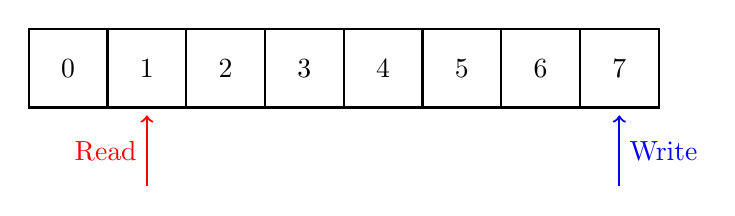
\begin{tikzpicture}
\foreach \i in {0,1,2,3,4,5,6,7} {
    \draw[thick] (\i,0) rectangle (\i+1,1); % Draw each spot in the queue
    \node at (\i+0.5, 0.5) {\i}; % Label each spot
}
\draw[thick, ->, red] (1.5, -1) -- (1.5, -0.1) node[midway, left] {Read};
\draw[thick, ->, blue] (7.5, -1) -- (7.5, -0.1) node[midway, right] {Write};
\end{tikzpicture}
\end{center}

Since the reader and writer execute in different contexts, the instructions in a read
and write can interleave in \textit{any} way imaginable:
\begin{itemize}
    \item Reader empty check can happen just as the writer is writing data
    \item Writer full check can happen just as the reader is reading data
    \item Reading and writing can occur concurrently
\end{itemize}

The key observation is the index held by the write pointer is reserved by the
writer. Similarly, the index held by the read pointer is reserved by the reader. The
only exception is when the read pointer equals to write pointer, then the queue is
empty. Given the possible ways the reader and writer execution can interleave, 
we can use TLA+ to verify the design.

\section{Spec}

TLA+ specification can be written using its native formal specification language,
or a C-like syntax called PlusCal (which transpires down to its native form).
In this example, I chose to implement the specification using PlusCal, since the
content to be verified is pseudo implementation. While it is possible to specify
SPSC in native TLA+, I find the approach more error-prone as each line is
effectively an individual state to be modeled.\newline

The following is a snippet of the \textit{Spec} written in PlusCal:\newline
\begin{ppcal}
procedure reader()
begin
r_chk_empty:        
    if rptr = wptr then 
    r_early_ret:            
        return;
    end if;
r_read_buf:         
    assert buffer[rptr] # 0;
r_cs:               
    buffer[rptr] := 0;
r_upd_rtpr:         
    rptr := (rptr + 1) % N;
    return;
end procedure; 
\end{ppcal}\newline
\begin{tlatex}
\@x{ {\p@procedure} reader ( )}%
\@x{ {\p@begin}}%
\@x{ r\_chk\_empty\@s{.5}\textrm{:}\@s{3}}%
\@x{\@s{16.4} {\p@if} rptr \.{=} wptr {\p@then}}%
\@x{\@s{16.4} r\_early\_ret\@s{.5}\textrm{:}\@s{3}}%
\@x{\@s{32.8} {\p@return} {\p@semicolon}}%
\@x{\@s{16.4} {\p@end} {\p@if} {\p@semicolon}}%
\@x{ r\_read\_buf\@s{.5}\textrm{:}\@s{3}}%
\@x{\@s{16.4} {\p@assert} buffer [ rptr ] \.{\neq} 0 {\p@semicolon}}%
\@x{ r\_cs\@s{.5}\textrm{:}\@s{3}}%
\@x{\@s{16.4} buffer [ rptr ] \.{:=} 0 {\p@semicolon}}%
\@x{ r\_upd\_rtpr\@s{.5}\textrm{:}\@s{3}}%
\@x{\@s{16.4} rptr \.{:=} ( rptr \.{+} 1 ) \.{\%} N {\p@semicolon}}%
\@x{\@s{16.4} {\p@return} {\p@semicolon}}%
\@x{ {\p@end} {\p@procedure} {\p@semicolon}}%
\end{tlatex}

\begin{ppcal}
procedure writer() 
begin
w_chk_full:         
    if (wptr + 1) % N = rptr then 
    w_early_ret:
        return; 
    end if;
w_write_buf:
    assert buffer[wptr] = 0;
w_cs:
    buffer[wptr] := wptr + 1000;
w_upd_wptr:
    wptr := (wptr + 1) % N;
    return;
end procedure; 
\end{ppcal}\newline
\begin{tlatex}
\@x{ {\p@procedure} writer ( )}%
\@x{ {\p@begin}}%
\@x{ w\_chk\_full\@s{.5}\textrm{:}\@s{3}}%
\@x{\@s{16.4} {\p@if} ( wptr \.{+} 1 ) \.{\%} N \.{=} rptr {\p@then}}%
\@x{\@s{16.4} w\_early\_ret\@s{.5}\textrm{:}\@s{3}}%
\@x{\@s{32.8} {\p@return} {\p@semicolon}}%
\@x{\@s{16.4} {\p@end} {\p@if} {\p@semicolon}}%
\@x{ w\_write\_buf\@s{.5}\textrm{:}\@s{3}}%
\@x{\@s{16.4} {\p@assert} buffer [ wptr ] \.{=} 0 {\p@semicolon}}%
\@x{ w\_cs\@s{.5}\textrm{:}\@s{3}}%
\@x{\@s{16.4} buffer [ wptr ] \.{:=} wptr \.{+} 1000 {\p@semicolon}}%
\@x{ w\_upd\_wptr\@s{.5}\textrm{:}\@s{3}}%
\@x{\@s{16.4} wptr \.{:=} ( wptr \.{+} 1 ) \.{\%} N {\p@semicolon}}%
\@x{\@s{16.4} {\p@return} {\p@semicolon}}%
\@x{ {\p@end} {\p@procedure} {\p@semicolon}}%
\end{tlatex}

\section{Safety}

Some safety requirement we can enforce include:\newline

\begin{tla}
MUTEX ==
    ~ ((pc[WRITER] = "w_cs") /\ (pc[READER] = "r_cs") /\ rptr = wptr)

Inv_Basics == 
    /\ ((written \cup writing) \cup unused) = all
    /\ reading \subseteq written                            \* reading is a subset of written
    /\ \A i \in unused : buffer[i] = 0
    /\ \/ Cardinality(to_be_read) + 1 = Cardinality(reading) 
       \/ Cardinality(to_be_read)     = Cardinality(reading) + 1
       \/ Cardinality(to_be_read)     = Cardinality(reading)
    /\ MUTEX
\end{tla}
\begin{tlatex}
\@x{ MUTEX \.{\defeq}}%
 \@x{\@s{16.4} {\lnot} ( ( pc [ WRITER ] \.{=}\@w{w\_cs} ) \.{\land} ( pc [
 READER ] \.{=}\@w{r\_cs} ) \.{\land} rptr \.{=} wptr )}%
\@pvspace{8.0pt}%
\@x{ Inv\_Basics \.{\defeq}}%
 \@x{\@s{16.4} \.{\land} ( ( written \.{\cup} writing ) \.{\cup} unused )
 \.{=} all}%
\@x{\@s{16.4} \.{\land} reading \.{\subseteq} written\@s{110.7}}%
\@y{%
  reading is a subset of written
}%
\@xx{}%
\@x{\@s{16.4} \.{\land} \A\, i \.{\in} unused \.{:} buffer [ i ] \.{=} 0}%
 \@x{\@s{16.4} \.{\land} \.{\lor} Cardinality ( to\_be\_read ) \.{+} 1 \.{=}
 Cardinality ( reading )}%
 \@x{\@s{16.4} \.{\lor} Cardinality ( to\_be\_read )\@s{16.4} \.{=}
 Cardinality ( reading ) \.{+} 1}%
 \@x{\@s{16.4} \.{\lor} Cardinality ( to\_be\_read ) \.{=} Cardinality (
 reading )}%
\@x{\@s{16.4} \.{\land} MUTEX}%
\end{tlatex}
\newline

\section{Liveness}

All indicies are eventually used:

\begin{tla}
    Liveness ==
    \A k \in 0..N-1:
    <>(buffer[k] # 0)
\end{tla}
\begin{tlatex}
\@x{\@s{16.4} Liveness \.{\defeq}}%
\@x{\@s{16.4} \A\, k \.{\in} 0 \.{\dotdot} N \.{-} 1 \.{:}}%
\@x{\@s{16.4} {\Diamond} ( buffer [ k ] \.{\neq} 0 )}%
\end{tlatex}

Unused index 0 becomes used, used index 0 becomes unused.
\begin{tla}
    Liveness2 ==
    /\ (buffer[0] = 0) ~> buffer[0] = 1000
    /\ (buffer[0] = 1000) ~> buffer[0] = 0
\end{tla}
\begin{tlatex}
\@x{\@s{16.4} Liveness2 \.{\defeq}}%
 \@x{\@s{16.4} \.{\land} ( buffer [ 0 ] \.{=} 0 ) \.{\leadsto} buffer [ 0 ]
 \.{=} 1000}%
 \@x{\@s{16.4} \.{\land} ( buffer [ 0 ] \.{=} 1000 ) \.{\leadsto} buffer [ 0 ]
 \.{=} 0}%
\end{tlatex}

% \end{document}

\* Add statements after this line.

SPECIFICATION Spec
\* INVARIANTS TypeOK NotSolved

CONSTANTS 
    N = 4
    READERS = {r0, r1}

INVARIANTS 
    Inv_Basics
    \* Inv_UniqueReaderPointers
    \* Inv_ReadingVsReady
    \* Inv_NonZeroCount
    \* Inv_UniqueReader
    \* Inv_DataValidity
    \* Inv_BufferSlotLifecycle
    \* Inv_ProducerConsumerSeparation
    \* Inv_DataValidity2

PROPERTIES 
    Liveness
    Liveness2

\* SYMMETRY 
\*     Perms


\part{Reference}


% \begin{document}

\chapter{Language}

Like other languages, TLA+ provides its data structure. I assume the readers are
already familiar with common data structure, and this chapter will only focus on
the TLA+ language semantics. 

\section{Data Structure}

\subsection{Set}

This is the most common data structure used in TLA+ spec. The following is a few examples on
how a set can be used:\newline
\begin{tla}
a == {0, 1, 2}
b == {2, 3, 4}
c == a \union b         \* \{0, 1, 2, 3, 4\}
d == a \intersect b     \* \{2\}
e == \E x \in c: x > 3  \* TRUE - because 4 in c is bigger than 3
f == \E x \in c: x > 5  \* FALSE - nothing in c is bigger than 5
g == \A x \in c: x < 3  \* FALSE - not all elements in c are smaller than 3
h == \A x \in c: x < 5  \* TRUE - all elements in c are smaller than 3
i == {x \in c: x < 3}   \* \{0, 1, 2\} - all elementse less than 3
j == Cardinality(c)     \* 5 - the number of elements in c
k == c \ d              \* \{0, 1, 3, 4\} - c substracts d
\end{tla}
\begin{tlatex}
\@x{ a\@s{0.26} \.{\defeq} \{ 0 ,\, 1 ,\, 2 \}}%
\@x{ b\@s{0.91} \.{\defeq} \{ 2 ,\, 3 ,\, 4 \}}%
\@x{ c\@s{0.97} \.{\defeq} a \.{\cup} b\@s{48.73}}%
\@y{%
  \{0, 1, 2, 3, 4\}
}%
\@xx{}%
\@x{ d \.{\defeq} a \.{\cap} b\@s{48.73}}%
\@y{%
  \{2\}
}%
\@xx{}%
\@x{ e\@s{0.79} \.{\defeq} \E\, x \.{\in} c \.{:} x \.{>} 3\@s{6.87}}%
\@y{%
  TRUE - because 4 in c is bigger than 3
}%
\@xx{}%
\@x{ f\@s{0.95} \.{\defeq} \E\, x \.{\in} c \.{:} x \.{>} 5\@s{6.87}}%
\@y{%
  FALSE - nothing in c is bigger than 5
}%
\@xx{}%
\@x{ g\@s{0.65} \.{\defeq} \A\, x \.{\in} c \.{:} x \.{<} 3\@s{6.87}}%
\@y{%
  FALSE - not all elements in c are smaller than 3
}%
\@xx{}%
\@x{ h\@s{0.26} \.{\defeq} \A\, x \.{\in} c \.{:} x \.{<} 5\@s{6.87}}%
\@y{%
  TRUE - all elements in c are smaller than 3
}%
\@xx{}%
\@x{ i\@s{2.05} \.{\defeq} \{ x \.{\in} c \.{:} x \.{<} 3 \}\@s{8.2}}%
\@y{%
  \{0, 1, 2\} - all elementse less than 3
}%
\@xx{}%
\@x{ j\@s{1.63} \.{\defeq} Cardinality ( c )\@s{16.4}}%
\@y{%
  5 - the number of elements in c
}%
\@xx{}%
\@x{ k\@s{0.46} \.{\defeq} c \.{\,\backslash\,} d\@s{51.30}}%
\@y{%
  \{0, 1, 3, 4\} - c substracts d
}%
\@xx{}%
\end{tlatex}

\subsection{Tuple}

\begin{tla}
A == <<0, 1, 2>>                    
B == <<2, 3, 4>>
C == A \o B                         \* tuple: 0, 1, 2, 2, 3, 4
D == Len(C)                         \* 6
E == \A x \in 1..Len(C) : C[x] # 10 \* TRUE - every C[x] is not 10
                                    \* First tuple element is at index 1 (not 0)
F == \E x \in 1..Len(C) : C[x] = 2  \* TRUE - there exists a C[x] that is 2
G == {x \in 1..Len(C) : C[x] = 2}   \* \{3, 4\} - when index is 3 or 4, C[x] = 2
\end{tla}
\begin{tlatex}
\@x{ A\@s{1.17} \.{\defeq} {\langle} 0 ,\, 1 ,\, 2 {\rangle}}%
\@x{ B\@s{0.54} \.{\defeq} {\langle} 2 ,\, 3 ,\, 4 {\rangle}}%
\@x{ C \.{\defeq} A \.{\circ} B\@s{104.04}}%
\@y{%
  tuple: 0, 1, 2, 2, 3, 4
}%
\@xx{}%
\@x{ D\@s{0.11} \.{\defeq} Len ( C )\@s{95.84}}%
\@y{%
  6
}%
\@xx{}%
 \@x{ E\@s{0.62} \.{\defeq} \A\, x \.{\in} 1 \.{\dotdot} Len ( C ) \.{:} C [ x
 ] \.{\neq} 10}%
\@y{%
  TRUE - every C[x] is not 10
}%
\@xx{}%
\@x{\@s{158.36}}%
\@y{%
  First tuple element is at index 1 (not 0)
}%
\@xx{}%
 \@x{ F\@s{0.75} \.{\defeq} \E\, x \.{\in} 1 \.{\dotdot} Len ( C ) \.{:} C [ x
 ] \.{=} 2\@s{6.87}}%
\@y{%
  TRUE - there exists a C[x] that is 2
}%
\@xx{}%
 \@x{ G \.{\defeq} \{ x \.{\in} 1 \.{\dotdot} Len ( C ) \.{:} C [ x ] \.{=} 2
 \}\@s{2.22}}%
\@y{%
  \{3, 4\} - when index is 3 or 4, C[x] = 2
}%
\@xx{}%
\end{tlatex}

\subsection{Function}

\section{Temporal Logic}



\chapter{Idiom}

Choose a x in set S such that for every Y in S x is smaller than y.
Finding minimum in set:\newline
\begin{tla}
    Min(S) == CHOOSE x \in S : \A y \in S : x <= y
\end{tla}
\begin{tlatex}
 \@x{\@s{16.4} Min ( S ) \.{\defeq} {\CHOOSE} x \.{\in} S \.{:} \A\, y \.{\in}
 S \.{:} x \.{\leq} y}%
\end{tlatex}
\newline

messages is an unordered map with untyped key and integer value:\newline

\begin{tla}
messages = [m \in {} |-> 0]
\end{tla}
\begin{tlatex}
\@x{ messages \.{=} [ m \.{\in} \{ \} \.{\mapsto} 0 ]}%
\end{tlatex}

\chapter{Fairness and Liveness}

For rigorous definition and proof, please refer to (TODO: citations). This
chapter focus on the application aspect of liveness and fairness and define an elevator 
spec that goes up and down.\newline

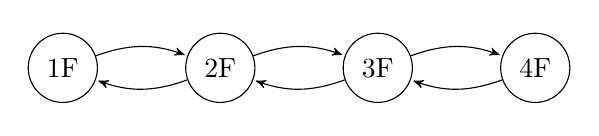
\begin{tikzpicture}[>=stealth',shorten >=1pt,auto,node distance=2cm]
  \node[state]  (q1)                {1F};
  \node[state]  (q2) [right of=q1]  {2F};
  \node[state]  (q3) [right of=q2]  {3F};
  \node[state]  (q4) [right of=q3]  {4F};

  \path[->]          (q1)  edge   [bend left=20]   node {} (q2);
  \path[->]          (q2)  edge   [bend left=20]   node {} (q1);

  \path[->]          (q2)  edge   [bend left=20]   node {} (q3);
  \path[->]          (q3)  edge   [bend left=20]   node {} (q2);

  \path[->]          (q3)  edge   [bend left=20]   node {} (q4);
  \path[->]          (q4)  edge   [bend left=20]   node {} (q3);

\end{tikzpicture}

\section{Liveness}

Consider the following elevator \textit{Spec}:
\begin{tla}
--------------------------- MODULE elevator ----------------------------
EXTENDS Integers
VARIABLES a
vars == <<a>>
TOP     == 4
BOTTOM  == 1
Init ==
    /\ a = BOTTOM
Up == 
    /\ a # TOP
    /\ a' = a + 1
Down == 
    /\ a # BOTTOM
    /\ a' = a - 1
Spec ==
  /\ Init
  /\ [][Up \/ Down]_a
=============================================================================
\end{tla}
\begin{tlatex}
\@x{}\moduleLeftDash\@xx{ {\MODULE} elevator}\moduleRightDash\@xx{}%
\@x{ {\EXTENDS} Integers}%
\@x{ {\VARIABLES} a}%
\@x{ vars \.{\defeq} {\langle} a {\rangle}}%
\@x{ TOP\@s{28.75} \.{\defeq} 4}%
\@x{ BOTTOM\@s{4.10} \.{\defeq} 1}%
\@x{ Init \.{\defeq}}%
\@x{\@s{16.4} \.{\land} a \.{=} BOTTOM}%
\@x{ Up \.{\defeq}}%
\@x{\@s{17.27} \.{\land} a \.{\neq} TOP}%
\@x{\@s{17.27} \.{\land} a \.{'} \.{=} a \.{+} 1}%
\@x{ Down \.{\defeq}}%
\@x{\@s{16.4} \.{\land} a \.{\neq} BOTTOM}%
\@x{\@s{16.4} \.{\land} a \.{'} \.{=} a \.{-} 1}%
\@x{ Spec \.{\defeq}}%
\@x{\@s{8.2} \.{\land}\@s{0.16} Init}%
\@x{\@s{8.2} \.{\land}\@s{0.16} {\Box} [ Up \.{\lor} Down ]_{ a}}%
\@x{}\bottombar\@xx{}%
\end{tlatex}

The building has a set of floors and the elevator can go either up or down. The
elevator keeps going up until it's the top floor, or keep going down until it's
the bottom floor. TLC will pass the \textit{Spec} as is.\newline

Let's introduce a liveness property. The elevator should always at least go 
to the second floor:\newline
\begin{tla}
Liveness == 
    /\ a = 1 ~> a = 2
\end{tla}
\begin{tlatex}
\@x{ Liveness \.{\defeq}}%
\@x{\@s{16.4} \.{\land} a \.{=} 1 \.{\leadsto} a \.{=} 2}%
\end{tlatex}
\newline

Running the \textit{Spec} against TLC will report a violation:

\begin{verbatim}
Error: Temporal properties were violated.
Error: The following behavior constitutes a counter-example:
State 1: <Initial predicate>
a = 1
State 2: Stuttering
\end{verbatim}

Since the \textit{Spec} permits \textit{suttering}, the state machine is allowed
to perpetually stay on 1F and \textit{never} go to 2F. This can be fixed by
introducing fairness description.

\section{Weak Fairness}

Weak fairness is defined as:\newline
\begin{equation} 
\Diamond\Box(ENABLED\langle A \rangle _v) \implies \Box\Diamond\langle A \rangle _v
\end{equation}
$ENABLED\langle A \rangle$ represents \textit{conditions required} for action A.
The above translates to: if conditions required for action A to occur is
\textit{eventually always} true, then action A will \textit{always eventually}
happen.\newline 

Without weak fairness defined, the elevator may \textit{stutter} at 1F and
never go to 2F. Weak fairness states that if the conditions of an action is
\textit{eventually always} true (ie. elevator decides to stay on 1F but 
\textit{can} go up), the elevator \textit{always eventually} go up.\newline

\begin{tla}
Spec ==
  /\ Init
  /\ [][Down \/ Up]_a
  /\ WF_a(Down)
  /\ WF_a(Up)
\end{tla}
\begin{tlatex}
\@x{ Spec \.{\defeq}}%
\@x{\@s{8.2} \.{\land}\@s{0.16} Init}%
\@x{\@s{8.2} \.{\land}\@s{0.16} {\Box} [ Down \.{\lor} Up ]_{ a}}%
\@x{\@s{8.2} \.{\land}\@s{0.16} {\WF}_{ a} ( Down )}%
\@x{\@s{8.2} \.{\land}\@s{0.16} {\WF}_{ a} ( Up )}%
\end{tlatex}
\newline

Running the spec against TLC passes again. What if we want to verify the
elevator eventually always goes to the top, not just to 2F? Let's modify the
Liveness property again:\newline
\begin{tla}
Liveness == 
    /\ a = BOTTOM ~> a = TOP
\end{tla}
\begin{tlatex}
\@x{ Liveness \.{\defeq}}%
\@x{\@s{16.4} \.{\land} a \.{=} BOTTOM \.{\leadsto} a \.{=} TOP}%
\end{tlatex}
\newline

TLC now reports the following violation: 
\begin{verbatim}
Error: Temporal properties were violated.
Error: The following behavior constitutes a counter-example:
State 1: <Initial predicate>
a = 1
State 2: <Up line 10, col 5 to line 11, col 17 of module elevator>
a = 2
Back to state 1: <Down line 13, col 5 to line 14, col 17 of module elevator>
\end{verbatim}

TLC identified a case where the elevator is perpetually stuck going between 1F
and 2F, but never go to 3F. Weak fairness is no longer enough, because the the
elevator is not stuck on 2F repeatedly, but stuck going between 1F and 2F. This
is where we need strong fairness.

\section{Strong Fairness}

Strong fairness is defined as:\newline
\begin{equation} 
\Box\Diamond(ENABLED\langle A \rangle _v) \implies \Box\Diamond\langle A \rangle _v
\end{equation}
The difference between weak and strong fairness is the \textit{eventually
always} vs. \textit{always eventually}. \newline 

In weak fairness, once the state machine is stuck in a state forever, the state
machine always transition to a possible next state permitted by the
\textit{Spec} (eg. if the elevator is stuck on 1F but can go to 2F, it will).
With strong fairness, the elevator doesn't need to be stuck on 2F to go to 3F.
If the elevator \textit{always eventually} makes it to 2F, it \textit{always
eventually} go to 3F.\newline 

Intuitively we are tempted to enable strong fairness like so: \newline
\begin{tla}
Spec ==
  /\ Init
  /\ [][Up \/ Down]_a
  /\ WF_a(Down)
  /\ SF_a(UP)
\end{tla}
\begin{tlatex}
\@x{ Spec \.{\defeq}}%
\@x{\@s{8.2} \.{\land}\@s{0.16} Init}%
\@x{\@s{8.2} \.{\land}\@s{0.16} {\Box} [ Up \.{\lor} Down ]_{ a}}%
\@x{\@s{8.2} \.{\land}\@s{0.16} {\WF}_{ a} ( Down )}%
\@x{\@s{8.2} \.{\land}\@s{0.16} {\SF}_{ a} ( UP )}%
\end{tlatex}
\newline 

However, TLC \textit{still} reports the same violation. What's going on?\newline

If we take a closer look at the enabling condition for \textit{Up}, it only
requires current floor to be not the \textit{top floor}. When the elevator is
stuck in a loop going Up and Down between 1F and 2F indefinitely, strong
fairness for Up is \textit{already satisfied}. What we really want is strong
fairness on \textit{Up} for \textit{every floor}, instead of \textit{any floor
except top floor}. So if elevator makes to 2F once, it will \textit{always
eventaully} go to 3F. If elevator makes to 3F once, it will \textit{always
eventaully} go to 4F, so on and so forth. The following is the change
required:\newline

\begin{tla}
Spec ==
  /\ Init
  /\ [][Up \/ Down]_a
  /\ WF_a(Down)
  /\ \A f \in BOTTOM..TOP-1: 
    /\ WF_a(Up /\ f = a)
\end{tla}
\begin{tlatex}
\@x{ Spec \.{\defeq}}%
\@x{\@s{8.2} \.{\land}\@s{0.16} Init}%
\@x{\@s{8.2} \.{\land}\@s{0.16} {\Box} [ Up \.{\lor} Down ]_{ a}}%
\@x{\@s{8.2} \.{\land}\@s{0.16} {\WF}_{ a} ( Down )}%
 \@x{\@s{8.2} \.{\land}\@s{0.16} \A\, f \.{\in} BOTTOM \.{\dotdot} TOP \.{-} 1
 \.{:}}%
\@x{\@s{16.4} \.{\land} {\WF}_{ a} ( Up \.{\land} f \.{=} a )}%
\end{tlatex}
\newline

Once again with this change TLC will pass.

\chapter{General Guideline}

\section{Model Checker Debug}

Debugging in TLC is a bit different than debugging with normal programs. A step
in the model checker is really a state transition. Even if the model cheker
completes, it's still worthwhile dump and audit the states just to make sure the
Spec is defined correctly.

\begin{verbatim}
tlc elevator -dump out > /dev/null && cat out.dump | head -n5
State 1:
a = 1
State 2:
a = 2
\end{verbatim}

You may want to grep the output to look for state being set to certain value to 
confirm the Spec is working as intended.

\subsection{Dead Lock}

Deadlock typically happens when the model checker ran out of things to do. This
is typically a result of an incomplete Spec definition, where certain edge cases
were not accounted for. The model checker typically provides a fairly
comprehensive backtrace leading up to the dead lock to simplify debug.

\subsection{Live Lock}

Livelock happens when the model checker identifies a case where the liveness
property is violated. An example is the elevator stuck going between two floors 
instead of keep going to the top floor, or the system is stuck dropping and
retransmit the same packet.\newline 

These are typically fixed by providing additional fairness description to the
Spec, telling the model checker how continue in the case of a live lock.\newline 

For a detail fairness description please refer to Chapter~\ref{chap:fairness}.

\section{Model Refinement}

This is, in some sense, the \textit{art} associated with writing model checker
verifiable TLA+ spec. Model checking is only valuable if it can be verified
within a reasonable amount of time. Since the model complexity grows
exponentially, there's little value in attempting to hyper-optimize the details.
Designer should focus on optimizing the broad stroke, such as removing features 
that are harder to get wrong, and focus the model on the bits that have the
highest return on investment.\newline

One useful way of trimming out low value portion of the Spec is to audit the
state dump. Even in the case of a non-terminating run, a partial state dump can
help identify low value details we can remove from the Spec.\newline

One key value of TLA+ is it highlights all the corner cases in the system. Even
if you end up removing certain details from the Spec, it still likely highlights
to you certain condition you were unaware of.\newline

As a broad stroke principle: when the Spec has millions or higher more states,
it is unlikely to terminate within a few seconds. From first principles if you
can find one failure case in a million states, you can also likely reduce the 
scope of the model to reproduce the failure in much fewer states.

\section{Liveness}

While safety properties can catch per state contradictions, liveness properties
allows you to verify the behaviour across a series of states. This is TLA+'s
\textit{super power}. We are rarely interested only in the correctness of one
state state in the system, but rather the correctness of system behaviour
\textit{across} a set of states. \newline

This book has already provided with a few examples of liveness properties: eg.
elevator eventually makes it to the top floor, consensus protocol eventually
converge, scheduling algorithm gaurantees a lock requester eventually gets the
lock, etc. I argue any system worth the reader's time to model using TLA+ must 
have interesting liveness properties to verify.\newline

Unfortunately, liveness check also takes \textit{much} longer, since the very
definition of verifying property across a series of states make the task very
hard to parallelize. Care must go into refining the model to keep the model
checker runtime reasonable.

\chapter{Reference}

\begin{thebibliography}{9}

\bibitem{ss}
Specifying Systems, 
https://lamport.azurewebsites.net/tla/book.html

\bibitem{toolbox}
TLA Toolbox,
https://github.com/tlaplus/tlaplus

\bibitem{tla_comm}
TLA+ Community Modules,
https://github.com/tlaplus/CommunityModules

\bibitem{}
Fairness in TLA+,
https://sriku.org/posts/fairness-in-tlaplus/
% \bibitem{}
% https://www.cds.caltech.edu/~murray/courses/afrl-sp12/L3_ltl-24Apr12.pdf
% Richard M. Murray, Nok Wongpiromsarn
% \textit{Linear Temporal Logic, Lecture 3}, 2012

\bibitem{backblaze}
Backblaze Durability Calculates at 99.999999999\% — And Why It Doesn’t Matter,
https://www.backblaze.com/blog/cloud-storage-durability/

\bibitem{raft}
In Search of an Understandable Consensus Algorithm,
https://raft.github.io/raft.pdf

\bibitem{raft_tla}
raft.tla,
https://github.com/ongardie/raft.tla

\bibitem{finite}
Wrangling monotonic systems in TLA+,
https://ahelwer.ca/post/2023-11-01-tla-finite-monotonic/

\bibitem{c10k}
C10k problem,
https://en.wikipedia.org/wiki/C10k\_problem

\bibitem{dining}
Dining Philosophers,
https://en.wikipedia.org/wiki/Dining\_philosophers\_problem

\end{thebibliography}



\chapter{Abstraction Guideline}


\end{document}
